%versi 2 (8-10-2016)
\chapter{Landasan Teori}
\label{chap:teori}

Pada bab ini akan dijelaskan landasan teori mengenai Node.js, Express.js, Socket.io, Canvas API, jQuery, dan HTML Content Template.

\section{Node.js}
\label{sec:Node.js}

Node.js adalah sebuah \textit{platform} atau lingkungan untuk menjalankan JavaScript pada \textit{web server} yang dibangun berdasarkan \textit{V8} \footnote{\url{https://v8.dev/}, diakses 22 November 2018} yang merupakan \textit{engine} JavaScript milik perusahaan \textit{Google} \cite{nodeFound:09:nodejsdocs}. Node.js memiliki model \textit{event-driven} yang artinya seluruh aksi akan dilakukan berdasarkan suatu \textit{event} yang dipancarkan, dan \textit{non-blocking} yang artinya suatu aksi dalam Node.js akan langsung dilakukan tanpa harus menunggu aksi sebelumnya selesai. 
%Teknologi ini menyediakan beberapa kelas yang berfungsi untuk mengimplementasi fitur-fitur yang dimiliki.

Seluruh berkas atau kelas yang ada di dalam Node.js dianggap sebagai modul-modul yang terpisah satu sama lain. Setiap modul memiliki atribut dan fungsi masing-masing. Modul-modul tersebut memiliki fitur yang berbeda-beda yang membantu pengembangan aplikasi web pada bagian \textit{server}. Strutkur modul yang ada pada Node.js dapat dilihat pada Gambar \ref{fig:nodejs_modul}.

\begin{figure}[H]
	\centering
	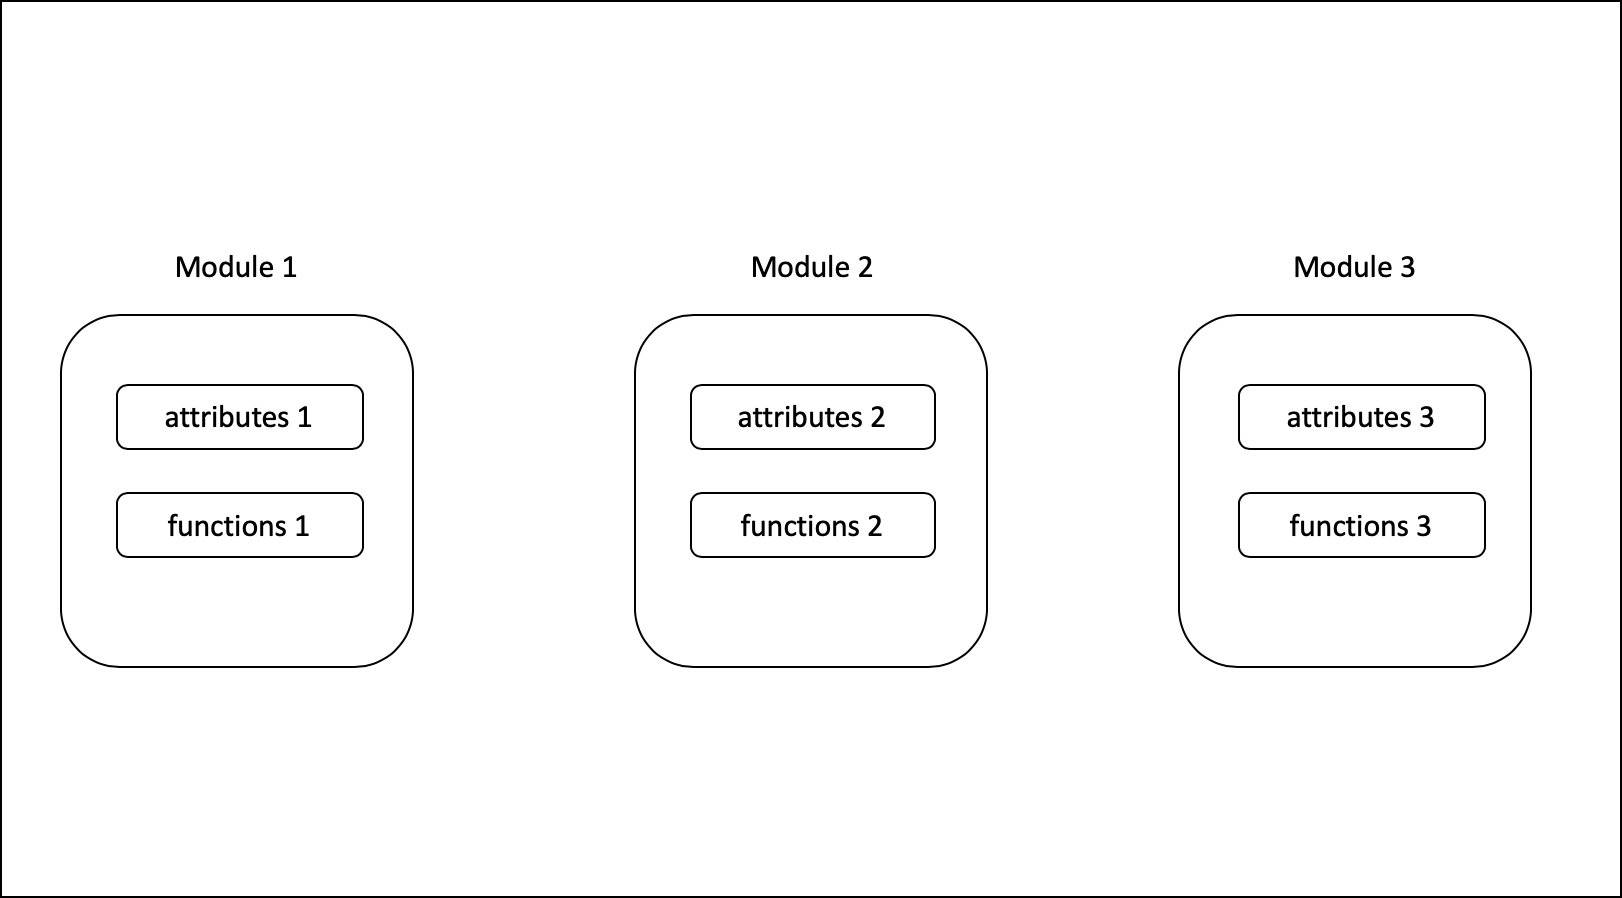
\includegraphics[scale=0.3]{Gambar/nodejs_modul}
	\caption{Struktur modul pada Node.js.}
	\label{fig:nodejs_modul}
\end{figure}

Komunikasi yang ada di dalam Node.js dilakukan dengan memancarkan suatu \textit{event}. Proses memancarkan suatu \textit{event} adalah pengiriman data yang dilakukan oleh satu pihak dengan menggunakan \textit{event}. Data yang ada di dalam \textit{event} tersebut akan terus disimpan. Apabila ada satu pihak yang membutuhkan data yang ada di dalam \textit{event} yang sudah dipancarkan maka pihak tersebut harus menggunakan fungsi tertentu untuk menangkap \textit{event} yang dibutuhkan. Proses bagaimana suatu \textit{event} bekerja dijelaskan sebagai berikut:

\begin{itemize}
	\item Apabila \textit{client} akan mengirim suatu data kepada \textit{server} maka \textit{client} akan memancarkan suatu \textit{event}.
	\item \textit{Event} yang telah dipancarkan akan menunggu untuk ditangkap oleh \textit{server}. \textit{Event} harus ditangkap dengan menggunakan fungsi tertentu.
	\item \textit{Server} akan menangkap \textit{event} yang telah dipancarkan oleh \textit{client}. Dengan begitu, data-data yang dikirimkan oleh \textit{client} telah berhasil didapatkan oleh \textit{server}.
	\item Apabila \textit{event} yang telah dipancarkan oleh \textit{client} tidak ditangkap oleh \textit{server} maka \textit{event} tersebut akan dihancurkan secara otomatis setelah satu sesi komunikasi selesai.
\end{itemize}

Subbab-subbab berikut menjelaskan beberapa modul yang dimiliki oleh Node.js.

\subsection{HTTP}
\textit{HTTP} merupakan suatu modul pada Node.js yang digunakan untuk menangani permintaan dari protokol HTTP. Modul ini akan menangani protokol HTTP dengan tidak melakukan \textit{buffer}. Hal tersebut berarti menyimpan sementara seluruh data yang akan dikirimkan pada seluruh permintaan atau respon.

Terdapat beberapa kelas yang mengimplementasi modul \textit{HTTP}. Berikut akan dijelaskan salah satu kelas yang mengimplementasi modul \textit{HTTP}.

\begin{enumerate}
%	\item \textbf{http.IncomingMessage} \\ 
%	Objek dari kelas ini akan dibuat oleh kelas \textit{http.Server} atau \textit{http.ClientRequest} dan memasukannya sebagai argumen suatu \textit{event} \textit{'request'} dan \textit{'response'}. Objek tersebut dapat digunakan untuk mengakses status \textit{response}, \textit{headers}, dan data. Kelas ini mengimplementasi \textit{interface Readable Stream}, beserta \textit{method, events,} dan properti yang ada didalamnya.
%	
%	\textbf{Properti:}
%	\begin{itemize}
%		\item \textbf{message.headers} \\ \textbf{Kembalian:} \textit{headers} milik objek \textit{request/response.}
%		\item \textbf{message.rawHeaders} \\ \textbf{Kembalian:} bentuk \textit{raw} dari \textit{headers} milik objek \textit{request/response}.
%		\item \textbf{message.statusCode} \\ \textbf{Kembalian:} tiga dijit kode status \textit{HTTP response}. Contoh: 404.
%		\item \textbf{message.statusMessage} \\ \textbf{Kembalian:} pesan status \textit{HTTP response} Contoh: \textit{OK} atau \textit{Internal Server Error.}
%		\item \textbf{message.url} \\ \textbf{Kembalian:} \textit{URL string} yang muncul pada permintaan \textit{HTTP}.
%	\end{itemize}
	
%	\item \textbf{http.ClientRequest} \\ 
%	Objek dari kelas ini dibuat dalam kelas ini sendiri dan dikembalikan dari \textit{method http.request()}. Objek ini merepresentasikan permintaan yang sedang berlangsung dimana \textit{header} objek tersebut sudah berada dalam antrian. \textit{Header} masih dapat diubah dengan menggunakan \textit{setHeader(name, value)} dan \textit{removeHeader(name)}. \textit{Header} yang asli akan dikirim bersamaan dengan \textit{chunk} pertama dari suatu data atau saat memanggil \textit{request.end()}.
%	
%	Beberapa \textbf{event} yang dimiliki oleh kelas ini yaitu sebagai berikut:
%	\begin{itemize}
%		\item \textbf{'connect'} \\ Dipancarkan saat \textit{server} merespon kepada permintaan.
%		\item \textbf{'response'} \\ Dipancarkan saat suatu respon diterima atas permintaan saat ini.
%		\item \textbf{'timeout'} \\ Dipancarkan saat suatu \textit{socket} telah mencapai batas waktu untuk tidak aktif.
%	\end{itemize}
%	
%	Beberapa \textit{method} yang dimiliki oleh kelas ini yaitu sebagai berikut:
%	\begin{itemize}
%		\item \textbf{request.end([data[,encoding]][,callback])} \\ 
%		\textbf{Parameter:} 
%		\begin{itemize}
%			\item \textbf{data} \\tipe: \textbf{string} atau \textbf{Buffer} \\ Data yang akan dikirim.
%			\item \textbf{encoding} \\tipe: \textbf{string} \\ Bersifat opsional dan akan bernilai \textit{utf8} apabila tipe parameter \textit{data} berupa \textit{string}.
%			\item \textbf{callback} \\tipe:	\textbf{Function} \\ Fungsi callback
%		\end{itemize}
%		
%		\textit{Method} ini akan mengakhiri proses pengiriman permintaan.
		
%		\item \textbf{request.getHeader(name)} \\
%		\textbf{Parameter:} 
%		\begin{itemize}
%			\item \textbf{name} \\tipe: \textbf{string} \\ Nama dari \textit{header} yang dibutuhkan.
%		\end{itemize}
%		\textbf{Kembalian:} suatu \textit{string} yang sesuai dengan parameter.
%		
%		\textit{Method} ini akan membaca seluruh \textit{header} dalam permintaan dan mengembalikan bagian yang sesuai dengan parameter. Berikut contoh implementasi dari \textit{method} ini:
%\begin{lstlisting}
%const contentType = request.getHeader('Content-Type');
%\end{lstlisting}
		
%		\item \textbf{request.removeHeader(name)} \\ 
%		\textbf{Parameter:}
%		\begin{itemize}
%			\item \textbf{name} \\tipe: \textbf{string} \\ Nama dari \textit{header} yang dibutuhkan.
%		\end{itemize}
%		\textit{Method} ini akan menghapus \textit{header} yang sudah ada pada objek \textit{header}. Berikut contoh implementasi dari \textit{method} ini:
%\begin{lstlisting}
%request.removeHeader('Content-Type');
%\end{lstlisting}
%		
%		\item \textbf{request.setHeader(name, value)} \\ 
%		\textbf{Parameter:}
%		\begin{itemize}
%			\item \textbf{name} \\tipe: \textbf{string} \\ Nama dari \textit{header} yang dibutuhkan.
%			\item \textbf{value} \\tipe: \textbf{value} \\ Nilai yang akan dimasukan pada objek \textit{header}
%		\end{itemize}
%		
%		\textit{Method} ini akan menetapkan suatu nilai kepada objek \textit{header}. Berikut contoh implementasi \textit{method} ini:
%\begin{lstlisting}
%request.setHeader('Content-Type', 'application/json');
%\end{lstlisting}
%	\end{itemize}
	
	\item \textbf{http.Server} \\ 
	Kelas ini akan menciptakan objek \textit{server} HTTP, yang akan menangani setiap permintaan yang dilakukan oleh \textit{client}. Salah satu \textit{Method} yang dimiliki oleh kelas ini adalah:
%	Kelas ini merupakan turunan dari \textit{net.Server}. \textit{Event} yang dimiliki kelas ini yaitu sebagai berikut:
%	\begin{itemize}
%		\item \textbf{'close'} \\ Dipancarkan apabila \textit{server} sudah ditutup.
%		
%	\end{itemize}
%	
%	Beberapa properti yang dimiliki oleh kelas ini yaitu:
%	\begin{itemize}
%		\item \textbf{server.listening} \\ Mengembalikan \textit{boolean} yang menandakan apakah \textit{server} melakukan proses \textit{listening} untuk suatu koneksi atau tidak.
%		
%		\item \textbf{server.maxHeadersCount} \\ Mengembalikan \textit{number} yang menandakan batas maksimum suatu \textit{headers} yang masuk. Nilai default dari properti ini yaitu 2000.
%		
%		\item \textbf{server.timeout} \\ Mengembalikan \textit{number} yang menandakan \textit{timeout} dalam milidetik.
%	\end{itemize}
%	
	\begin{itemize}
		\item \textbf{server.listen()} \\ \textit{Method} ini akan memulai \textit{server} HTTP untuk melakukan proses \textit{listening} suatu koneksi. Dengan begitu, \textit{server} akan mengetahui apabila ada \textit{client} yang melakukan permintaan untuk suatu koneksi.
	\end{itemize}
%		\item \textbf{server.setTimeout([msecs][,callback])} \\ \textbf{Parameter:}
%		\begin{itemize}
%			\item \textbf{msec} nilai \textit{timeout} dalam milidetik. secara default bernilai 120000 (2 menit).
%			\item \textbf{callback} fungsi \textit{callback}.
%		\end{itemize}
%		\textbf{Kembalian:} objek \textit{server}.
%		
%		\textit{Method} ini menetapkan nilai \textit{timeout} untuk \textit{sockets} dan memancarkan \textit{event 'timeout'} pada objek \textit{Server}.
%		
%		\item \textbf{server.close([callback])} \\ \textbf{Parameter:}
%		\begin{itemize}
%			\item \textbf{callback} fungsi \textit{callback}.
%		\end{itemize} 
%		
%		\textit{Method} ini menghentikan \textit{server} untuk menerima koneksi baru.
%	\end{itemize}
\end{enumerate} 

Modul \textit{HTTP} memiliki beberapa \textit{method} yang akan membantu dalam proses pengembangan suatu aplikasi. Salah satu \textit{method} yang dimiliki oleh \textit{HTTP} adalah sebagai berikut:
\begin{itemize}
	\item \textbf{http.createServer([options][,requestListener])} \\ 
	\textbf{Parameter:}
	\begin{itemize}
		\item \textbf{options} objek-objek seperti berikut:
			\begin{itemize}
				\item \textbf{IncomingMessage}, suatu kelas yang akan menciptakan objek \textit{request} yang merepresentasikan suatu permintaan yang dikirimkan oleh \textit{client}.
				
				\item \textbf{ServerResponse}, suatu kelas yang akan menciptakan objek \textit{response} yang merepresentasikan suatu respon yang dikirimkan oleh \textit{server}.
			\end{itemize}
			
		\item \textbf{requestListener} fungsi yang akan dieksekusi secara otomatis apabila \textit{event 'request'} dipancarkan. \textit{Event} tersebut menandakan bahwa \textit{client} telah melakukan suatu permintaan kepada \textit{server}
	\end{itemize}
	\textbf{Kembalian:} objek \textit{http.Server}
	
	\textit{Method} ini akan membuat objek \textit{http.Server} untuk menangani permintaan dari \textit{client} dan memberikan respon kepada \textit{client}. Fungsi yang diberikan pada \textit{method} ini akan dipanggil satu kali pada saat setiap permintaan yang dikirimkan kepada \textit{server}.
	
%	\item \textbf{http.request(options[,callback])} \\ 
%	\textbf{Parameter:}
%	\begin{itemize}
%		\item \textbf{options} \\ Dapat berupa \textit{Object, string} atau \textit{URL}. Berikut jenis-jenis \textit{options} yang dapat menjadi parameter:
%		\begin{itemize}
%			\item \textbf{protocol} \\tipe: \textbf{string} \\ Protokol yang digunakan.
%			\item \textbf{host} \\tipe: \textbf{string} \\ Nama domain atau alamat \textit{IP} milik server.
%			\item \textbf{hostname} \\tipe: \textbf{string} \\ Nama lain untuk \textit{host}.
%			\item \textbf{port} \\tipe: \textbf{number} \\ \textit{Port} untuk \textit{server}.
%			\item \textbf{path} \\tipe: \textbf{string} \\ \textit{Path} untuk permintaan.
%			\item \textbf{headers} \\tipe: \textbf{Object} \\ Objek yang berisi permintaan \textit{headers}.
%			\item \textbf{timeout} \\tipe: \textbf{number} \\ Nomor yang menentukan \textit{timeout} dari suatu \textit{socket} dalam milidetik.
%		\end{itemize}
%		
%		\item \textbf{callback} \\tipe: \textbf{Function} \\ Fungsi \textit{callback}.
%	\end{itemize}
%	
%	\textbf{Kembalian:} objek dari kelas \textit{http.ClientRequest}.
%	
%	\textit{Method} ini digunakan untuk menangani permintaan \textit{HTTP} pada \textit{server}. Berikut contoh implementasi dari \textit{method} ini:
%	\begin{lstlisting}
%	const options = {
%	hostname: 'www.google.com',
%	port: 80,
%	path: '/upload',
%	method: 'POST',
%	headers: {
%	'Content-Type': 'application/x-www-form-urlencoded',
%	'Content-Length': Buffer.byteLength(postData)
%	}
%	};
%	
%	const req = http.request(options, (res) => {
%	console.log(`STATUS: ${res.statusCode}`);
%	console.log(`HEADERS: ${JSON.stringify(res.headers)}`);
%	res.setEncoding('utf8');
%	res.on('data', (chunk) => {
%	console.log(`BODY: ${chunk}`);
%	});
%	res.on('end', () => {
%	console.log('No more data in response.');
%	});
%	});
%	
%	req.end();
%	\end{lstlisting}
	
\end{itemize}

\subsection{Path}
\textit{Path} adalah suatu modul yang menyediakan fungsi untuk mengatur akses suatu berkas dan direktori. Modul ini akan menunjukan suatu \textit{path} dalam bentuk \textit{string} yang dapat diakses oleh modul-modul lain.

%Modul tersebut dapat diakses dengan cara sebagai berikut:
%
%\begin{lstlisting}[caption={Akses modul \textit{path}}, label={lst:modulPath}, captionpos=b]
%const path = require('path');
%\end{lstlisting}
%
%Dengan cara tersebut, maka variabel \textit{path} akan mendapatkan kumpulan fungsi yang dimiliki oleh \textit{Path}. Dengan begitu, variabel tersebut dapat memanggil setiap \textit{method} milik \textit{Path} yang diperlukan. 

Salah satu method yang dimiliki oleh \textit{Path} adalah sebagai berikut: 

\begin{itemize}
	\item \textbf{path.join([...paths])} \\ 
	\textbf{parameter:} 
	\begin{itemize}
		\item \textbf{...paths} \\ tipe: \textbf{String} \\ Urutan suatu lokasi berkas yang akan digunakan.
	\end{itemize}

	\textbf{kembalian:} String
	
	\textit{Method} ini akan menggabungkan seluruh bagian-bagian \textit{path} dengan menormalisasinya dan mengembalikan bentuk \textit{path} yang menyeluruh.
\end{itemize}

%\subsection{Events}
%\textit{Node.js} dibangun berdasarkan arsitektur \textit{event-driven} dengan sifat \textit{asynchronous}, dimana jenis-jenis objek tertentu akan memancarkan suatu \textit{events} secara berkala dan akan memanggil objek \textit{Function} ("\textit{listeners}").
%
%Semua objek yang memancarkan \textit{events} merupakan turunan dari kelas \textit{EventEmitter}. Objek tersebut akan memanggil \textit{method} \textit{eventEmitter.on()} yang memungkinkan satu atau beberapa fungsi dapat ditangani dalam suatu \textit{event} yang dipancarkan oleh objek saat ini.
%
%Kelas \textit{EventEmitter} dapat didefinisikan dengan memanggil modul \textit{events} seperti berikut :
%
%\begin{lstlisting}
%const EventEmitter = require('events');
%\end{lstlisting}
%
%Sebuah \textit{EventEmitter} akan memancarkan \textit{'event'} \textit{'newListener'} pada saat \textit{listeners} baru akan ditambahkan, dan \textit{'removeListener'} akan dipancarkan saat \textit{listeners} saat ini akan dihapus.
%
%Berikut merupakan beberapa \textit{method} yang dimiliki oleh kelas \textit{EventEmitter}:
%
%\begin{itemize}
%	\item \textbf{eventEmitter.on(eventName, listener)} \\ \textbf{Parameter:}
%	\begin{itemize}
%		\item \textit{eventName}, nama dari suatu \textit{event} yang akan dipancarkan.
%		\item \textit{listener}, suatu fungsi \textit{callback} yang akan menangani \textit{event} dari \textit{eventName}. 
%	\end{itemize} 
%	\textbf{Kembalian:} referensi kepada \textit{EventEmitter}.
%	
%	\textit{Method} ini berfungsi untuk mencatat suatu listener yang akan digunakan. Fungsi \textit{listener} yang menjadi parameter \textit{method} ini akan ditambahkan ke \textit{index} terakhir dari \textit{array of listeners} pada \textit{eventName}. Tidak akan ada pengecekan apakah fungsi \textit{listener} sudah dimasukan sebelumnya. Oleh karena itu, pemanggilan \textit{eventName} dan \textit{listener} secara berulang akan menyebabkan fungsi \textit{listener} dimasukan kedalam \textit{array} dan dipanggil secara berulang. \textit{Method} ini juga akan mengembalikan \textit{reference} kepada \textit{EventEmitter}, sehingga pemanggilan dapat saling menyambung dengan pemanggilan lainnya.
%	
%	Berikut merupakan contoh implementasi dari \textit{method} ini:
%\begin{lstlisting}
%const EventEmitter = require('events');
%	
%class MyEmmit extends EventEmitter {}
%	
%const myEmmit = new MyEmitter();
%	
%myEmmit.on('event', () => {
%console.log('suatu event telah terjadi');	
%});
%\end{lstlisting}
%	
%	\item \textbf{eventEmitter.emit(eventName)} \\ \textit{Method} ini berfungsi untuk memicu suatu \textit{event} yang akan dipancarkan. \textbf{Parameter:}
%	\begin{itemize}
%		\item \textit{eventName}, nama dari sebuah \textit{event} yang akan dipancarkan.
%		\item \textit{...args}, argumen tambahan yang akan diberikan pada \textit{eventName}. 
%	\end{itemize}
%	\textbf{Kembalian:} \textit{true} apabila \textit{event} memiliki \textit{listener}, false jika tidak.
%	
%	\textit{Method} ini akan memanggil masing-masing \textit{listener} yang sudah dicatat oleh \textit{eventEmitter.on()} dalam \textit{array of listeners} secara sinkronis, dimana beberapa \textit{listener} tersebut mengacu pada \textit{eventName} yang sama. Argumen yang diterima dari parameter akan diberikan pada masing-masing \textit{listener}.
%	
%	Berikut merupakan contoh implementasi dari \textit{method} ini:
%\begin{lstlisting}
%const EventEmitter = require('events');
%	
%class MyEmmit extends EventEmitter {}
%	
%const myEmmit = new MyEmitter();
%	
%myEmmit.on('event', () => {
%console.log('suatu event telah terjadi');	
%});
%myEmitter.emit('event');
%\end{lstlisting} 
%\end{itemize}

%\subsection{Stream}
%Kelas ini digunakan untuk menangani aliran data yang terjadi pada \textit{Node.js}. Data yang ditangani dapat berjumlah banyak dan akan menghabiskan banyak memori apabila tidak ditangani dengan baik. Oleh karena itu, modul \textit{stream} menyediakan fitur-fitur yang memudahkan penanganan aliran data.
%
%Ada empat tipe dasar \textit{stream} dalam \textit{Node.js}:
%\begin{itemize}
%	\item \textbf{Readable} \\ \textit{Streams} yang dapat membaca data dari sumber eksternal tertentu.
%	\item \textbf{Writable} \\ \textit{Streams} yang dapat menulis data dan mengirimkannya ke sumber external tertentu.
%	\item \textbf{Duplex} \\ \textit{Streams} yang dapat membaca dan menulis data sekaligus.
%	\item \textbf{Transform} \\ \textit{Duplex streams} yang dapat memodifikasi atau mengubah data dimana data tersebut dapat dilihat langsung hasil perubahannya.
%\end{itemize}
%
%\begin{enumerate}
%	\item \textbf{Readable Stream} \\
%	Merupakan abstraksi untuk sumber data yang digunakan. Berikut merupakan contoh dari \textit{Readable Stream} pada \textit{Node.js}:
%	\begin{itemize}
%		\item \textbf{HTTP responses} pada \textit{client}
%		\item \textbf{HTTP requests} pada \textit{server}
%		\item \textbf{fs read streams}
%	\end{itemize}
%	Seluruh \textit{Readable streams} mengimplementasi \textit{interface} yang didefinisikan oleh kelas \textit{stream.Readable}.
%	
%	\begin{itemize}
%		\item \textbf{stream.Readable} \\
%		\textbf{Events:}
%		\begin{itemize}
%			\item \textbf{'close'} \\ \textit{Event} ini dipancarkan saat suatu \textit{stream} atau sumber lain telah ditutup. \textit{Event} ini menandakan tidak akan ada \textit{event} lagi yang akan dipancarkan, dan tidak ada komputasi lain yang akan dilakukan.
%\begin{lstlisting}
%const readable = getReadableStreamSomehow();
%readable.on('close', (chunk) => {
%console.log(`Stream telah ditutup`);
%});
%			\end{lstlisting}
%			
%			\item \textbf{'data'} \\ \textit{Event} ini akan dipancarkan setiap kali suatu \textit{stream} melepas kepemilikan sebuah data kepada pemakai. Hal tersebut dapat terjadi setiap suatu \textit{stream} berganti menjadi mode \textit{flowing} dengan memanggil \textit{readable.pipe()}, \textit{readable.resume()}, atau dengan menghubungkan \textit{listener callback} pada \textit{'data' event}. Contoh implementasi:
%\begin{lstlisting}
%const readable = getReadableStreamSomehow();
%readable.on('data', (chunk) => {
%console.log(`Menerima data sebesar ${chunk.length} bytes.`);
%});
%			\end{lstlisting}
%			
%			\item \textbf{'end'} \\ \textit{Event} ini dipancarkan saat tidak ada lagi data yang akan digunakan dari \textit{stream}. Contoh implementasi:
%\begin{lstlisting}
%const readable = getReadableStreamSomehow();
%readable.on('end', () => {
%console.log('Tidak akan ada data yang dikirimkan.');
%});
%\end{lstlisting}
%			
%			\item \textbf{'error'} \\ \textit{Event} ini akan dipancarkan oleh \textit{Readable} setiap saat. \textit{Event} ini dapat terjadi apabila \textit{stream} tidak dapat menyediakan data dikarenakan kesalahan internal, atau ketika implementasi suatu \textit{stream} mencoba mengirimkan \textit{chunk} dari data yang tidak sesuai. Contoh implementasi:
%\begin{lstlisting}
%const readable = getReadableStreamSomehow();
%readable.on('error', () => {
%console.error('Terjadi kesalahan');
%});
%\end{lstlisting}
%			
%			
%		\end{itemize}
%		
%		\textbf{Method:}
%		\begin{itemize}
%			\item \textbf{readable.pipe(destination[, options])} \\ \textbf{Parameter:}
%			\begin{itemize}
%				\item \textbf{destination} \\tipe: \textit{stream.Writable} \\ Destinasi untuk menulis suatu data.
%				\item \textbf{options} \\tipe: \textit{Object} \\ Bersifat opsional, dapat berupa objek sebagai berikut:
%				\begin{itemize}
%					\item \textbf{end} \\tipe: \textit{boolean} \\ Mengakhiri \textit{writer} yang melakukan proses menulis saat \textit{reader} telah selesai. Nilai \textit{default} parameter ini yaitu \textit{true}.
%				\end{itemize}
%			\end{itemize}
%			\textbf{Kembalian:} referensi yang menuju \textit{destination}.
%			
%			\textit{Method} ini akan menghubungkan \textit{Writable stream} pada objek \textit{readable}, sehingga dapat berubah menjadi mode \textit{flowing} secara otomatis dan akan menaruh seluruh data pada \textit{Writable} yang sudah terhubung. \textit{Method} ini mengembalikan referensi yang menuju \textit{destination}, sehingga \textit{pipe streams} dapat saling menyambung dengan \textit{pipe streams} lainnya.
%			
%			Berikut merupakan contoh implementasi dari \textit{method} ini:
%\begin{lstlisting}
%const fs = require('fs');
%			
%const readable = getReadableStreamSomehow();
%const writable = fs.createWriteStream('file.txt');
%			
%//seluruh data dari objek readable masuk ke 'file.txt'
%readable.pipe(writable); 
%\end{lstlisting}
%			
%		\end{itemize}
%	\end{itemize}
%\end{enumerate}

\subsection{Module}
Pada aplikasi berbasis Node.js, setiap berkas yang terdapat dalam pembangunan aplikasi dianggap sebagai modul-modul yang terpisah satu sama lain. Variabel dan fungsi yang terdapat pada satu berkas, atau modul, hanya dapat digunakan pada satu lingkup modul tersebut. Suatu modul tidak dapat menggunakan variabel atau fungsi yang terdapat pada modul lainnya. Oleh karena itu, apabila variabel dan fungsi yang terdapat pada satu modul dapat digunakan oleh modul yang lain, diperlukan cara tertentu. Cara tersebut dapat dilakukan seperti berikut:

\begin{lstlisting}[caption={Proses \textit{export} fungsi dan objek dari satu modul ke modul lain}, label={lst:modulExport}, captionpos=b, frame=single]
module.exports = functions || object
\end{lstlisting}

\textit{module.exports} merupakan objek yang dibentuk oleh sistem \textit{Module}. \textit{Functions} dan \textit{object} merupakan fungsi dan objek yang merupakan elemen-elemen dari modul tertentu, yang diubah menjadi global agar dapat diakses oleh modul lain. Dengan menggunakan cara ini, suatu modul dapat berubah menjadi global dan dapat diakses oleh modul-modul lain.

%------------- END OF NODE.JS --------------

\section{Express.js}
\label{sec:Express.js}

Express.js adalah suatu \textit{framework} untuk membangun aplikasi web yang berjalan berdasarkan Node.js \cite{nodeFound:10:expressjsapi}. Fitur-fitur yang ada pada Express.js digunakan untuk mengatur struktur direktori dalam pengembangan aplikasi web, sehingga untuk proses pemeliharaan aplikasi web dapat dilakukan secara efisien. Express.js memiliki beberapa fitur dan proses yang dapat membantu pengembangan aplikasi web. Fitur dan proses tersebut akan dijelaskan sebagai berikut:

\begin{itemize}
	\item \textbf{Middleware} \\ 
	\textit{Middleware} adalah fungsi yang memiliki akses terhadap seluruh permintaan dari \textit{client}, yang dapat memodifikasi permintaan tersebut sebelum mengirimkan respon kembali kepada \textit{client}. Beberapa hal yang dapat dilakukan oleh \textit{middleware} adalah sebagai berikut:
	\begin{itemize}
		\item Mengeksekusi perintah kode yang ada di dalam fungsi.
		\item Memodifikasi objek \textit{request} yang didapat dari \textit{client} dan \textit{response} yang akan diberikan kepada \textit{client}.
		\item Mengakhiri siklus \textit{request-response} yang artinya sudah tidak akan ada lagi permintaan dari \textit{client} dan respon dari \textit{server}.
		\item Memanggil fungsi \textit{next()} dimana fungsi tersebut akan memanggil fungsi \textit{middleware} selanjutnya yang ada di dalam program.
	\end{itemize}
%	Contoh bentuk fungsi \textit{middleware} akan dijelaskan sebagai berikut:
%\begin{lstlisting}[caption={Contoh fungsi \textit{middleware}}, label={lst:contohMiddleware}, captionpos=b]
%var express = require('express');
%var app = express();
%
%app.get('/', function(req, res, next){
%	next();
%})
%\end{lstlisting}
%	\textit{Middleware} adalah fungsi yang memiliki parameter \textit{req, res}, dan \textit{next}. Bagian-bagian parameter akan dijelaskan sebagai berikut:
%	\begin{itemize}
%		\item \textbf{req}, argumen yang merepresentasikan \textit{request} HTTP. Argumen ini dinamakan \textit{req} berdasarkan konvensi.
%		
%		\item \textbf{res}, argumen yang merepresentasikan \textit{response} HTTP. Argumen ini dinamakan \textit{res} berdasarkan konvensi.
%		
%		\item \textbf{next}, argumen \textit{callback} yang akan dieksekusi berdasarkan kondisi tertentu yang dapat ditentukan. \textit{Callback} adalah fungsi yang berperan sebagai argumen pada parameter fungsi lain. Argumen ini dinamakan \textit{next} berdasarkan konvensi.
%	\end{itemize}
	\item \textbf{Routing} \\
	\textit{Routing} adalah proses yang menentukan bagaimana suatu aplikasi akan memberikan respon pada saat \textit{client} mengakses \textit{URI(Unifor Resource Identifier)} milik aplikasi. Proses ini dapat dilakukan dengan menggunakan \textit{method} milik kelas \textit{Application} yang sesuai dengan \textit{method} dari protokol HTTP. Dengan adanya proses \textit{routing} maka aplikasi dapat menentukan respon yang sesuai dengan permintaan yang dilakukan oleh \textit{client}.
%	Berikut merupakan contoh penggunaan proses \textit{routing}:
%	
%	\begin{lstlisting}[caption={Contoh penggunaan proses \textit{routing}}, label={lst:routingEx}, captionpos=b]
%		var express = require('express');
%		var app = express();
%		
%		app.get('/', function(req, res){
%			res.send('GET request to the homepage');
%		});
%		
%		app.post('/', function(req, res){
%			res.send('POST request to the homepage');
%		});
%	\end{lstlisting}
%	
%	Proses \textit{routing} dilakukan pada saat ada permintaan dari \textit{client} yang menggunakan \textit{method} \textit{GET} dan \textit{POST}. Apabila menggunakan \textit{GET}, maka \textit{server} akan memberi respon dengan menampilkan teks \textit{'GET request to the homepage'}. Apabila menggunakan \textit{POST}, maka \textit{server} akan memberi respon dengan menampilkan teks \textit{'POST request to the homepage'}.
\end{itemize}
Express.js memiliki Beberapa kelas dengan fitur yang berbeda-beda untuk membantu pengembangan aplikasi web berbasis Node.js. Subbab-subbab berikut akan menjelaskan kelas-kelas yang terdapat pada Express.js.

\subsection{express()}
\label{subsec:express()}
Kelas ini dibutuhkan untuk mengakses seluruh fitur yang disediakan oleh Express.js. Untuk dapat mengakses seluruh fitur Express.js, langkah yang harus dilakukan adalah sebagai berikut: 
\begin{lstlisting}[caption={Mengakses fitur \textit{express()}}, label={lst:express()}, captionpos=b, frame=single]
var express = require('express');
\end{lstlisting}
Variabel \textit{express} digunakan untuk memuat seluruh fitur yang dimiliki oleh modul \textit{'express'}, sehingga variabel tersebut dapat menggunakan seluruh fitur yang tersedia. Dengan melakukan langkah tersebut, fitur-fitur yang terdapat pada Express.js sudah dapat digunakan untuk pengembangan aplikasi web.

Beberapa \textit{method} yang dimiliki oleh kelas \textit{express()} adalah sebagai berikut:
%Variabel \textit{app} akan melakukan proses instansiasi objek dari variabel \textit{express} dengan menetapkan fungsi \textit{express()}.

\begin{itemize}
%	\item \textbf{express.Router([options])} \\ \textbf{Parameter:} 
%	\begin{itemize}
%		\item \textbf{options} bersifat opsional dan akan menentukan sifat dari objek \textit{router}. Parameter ini dapat berupa beberapa jenis seperti berikut:
%		\begin{itemize}
%			\item \textit{caseSensitive} memungkinkan \textit{case-sensitive}. Dapat bernilai \textit{true} atau \textit{false}. Secara default akan bernilai \textit{false}.
%			
%			\item \textit{strict} memungkinkan \textit{strict routing}. Dapat bernilai \textit{true} atau \textit{false}. Apabila bernilai \textit{false}, maka parameter \textit{'/foo'} dan \textit{'/foo/'} akan dianggap sama oleh \textit{router}.
%		\end{itemize}
%	\end{itemize}

	\item \textbf{express.static(root, [,options])} \\
	\textbf{Parameter:}
	\begin{itemize}
		\item \textbf{root} \\ tipe: \textbf{String} \\ Menentukan direktori sumber utama yang akan digunakan untuk menyediakan berkas yang memiliki sifat statis. Berkas yang memiliki sifat statis dapat dikirimkan kepada \textit{client} tanpa harus dibangkitkan, dimodifikasi, atau dilakukan proses tertentu terlebih dahulu.
		\item \textbf{options} \\ Suatu objek seperti berikut:
			\begin{itemize}
				\item \textbf{dotfiles}, menentukan bagaimana mengatasi suatu \textit{dotfiles} (suatu berkas atau direktori yang dimulai dengan tanda ".").
			\end{itemize}
	\end{itemize}
	
	\textit{Method} ini menyediakan cara agar dapat mengakses berkas yang memiliki sifat statis. Berkas tersebut disimpan dalam suatu direktori lokal yang dapat diakses didalam proses pengembangan aplikasi web.
	
	\item \textbf{express.Router([options])} \\
	\textbf{Parameter:}
	\begin{itemize}
		\item \textbf{options} merupakan parameter pilihan yang akan menentukan perilaku dari \textit{server} pada saat diakses oleh \textit{client}. Parameter dapat berupa objek berikut ini:
		\begin{itemize}
			\item \textbf{caseSensitive} membedakan huruf besar dan huruf kecil.
		\end{itemize}
	\end{itemize}

	\textit{Method} ini akan membuat objek \textit{router} yang dapat digunakan untuk menangani permintaan dari \textit{client} pada saat \textit{client} mengakses \textit{URI} tertentu.
	 
	
\end{itemize}

\subsection{Application}
\label{subsec:application}
%
%Objek dari kelas ini akan menangani beberapa hal seperti berikut:
%
%\begin{itemize}
%	\item Proses \textit{routing}. \\
%	Proses ini mengatur respon yang akan diberikan saat suatu \textit{client} mengakses \textit{URI (Uniform Resource Identifier)}, yang merupakan alamat dari suatu aplikasi tertentu.
%	
%	\item Mengatur jalannya \textit{middleware}.  \\
%	\textit{Middleware} adalah suatu fungsi yang memiliki akses pada objek-objek yang berada didalam siklus \textit{request-response} aplikasi tertentu. Objek-objek tersebut adalah objek \textit{Request (req)}, objek \textit{Response (res)}, dan fungsi \textit{next},
%\end{itemize}
Kelas ini akan mengatur bagaimana perilaku aplikasi terhadap berbagai permintaan yang dilakukan oleh \textit{client}. Objek yang diciptakan dari kelas \textit{Application} dapat melakukan beberapa hal seperti berikut:
\begin{itemize}
	\item Proses \textit{routing} terhadap permintaan HTTP.
	\item Mengatur berjalannya \textit{middleware}.
	\item Melakukan proses \textit{rendering} pada berkas HTML.
	\item Mendaftarkan \textit{template engine} tertentu, yang digunakan untuk mengubah elemen-elemen HTML.
\end{itemize}

%Kelas ini akan menangani berbagai proses yang terjadi dalam aplikasi Express seperti melakukan proses \textit{routing} terhadap \textit{HTTP requests}, mengatur berjalannya \textit{middleware}, \textit{rendering} sebuah \textit{HTML views}, dan mendaftarkan \textit{template engine} tertentu.
%Objek dari kelas \textit{Application} dapat diciptakan dengan langkah seperti berikut:
%\begin{lstlisting}[caption={Mengakses fitur \textit{application}}, label={lst:expressApp}, captionpos=b]
%const express = require('express');
%const app = express();
%\end{lstlisting}
%
%Baris pertama dari potongan kode tersebut berarti variabel \textit{express} yang memanggil modul \textit{'express'} agar dapat mengakses fungsi-fungsi yang ada pada modul tersebut. Sedangkan baris kedua, Objek \textit{app} memanggil fungsi \textit{express()} yang telah didapatkan dari variabel \textit{express}. Dengan begitu, variabel \textit{app} dapat mengakses fungsi-fungsi yang ada didalam pengembangan aplikasi web.

Kelas ini memiliki beberapa \textit{method} sebagai berikut:

\begin{itemize}
%	\item \textbf{app.all(path, callback[, callback ...])} \\ \textbf{Parameter:} 
%	\begin{itemize}
%		\item \textbf{path} suatu \textit{path} yang akan ditangani oleh \textit{middleware}. Dapat berupa \textit{string}, \textit{path pattern}, atau \textit{array} dari kombinasi \textit{string} dan \textit{path pattern}.
%		
%		\item \textbf{callback} merupakan fungsi \textit{callback}, dimana fungsi tersebut dapat berupa fungsi \textit{middleware}, kumpulan dari fungsi \textit{middleware} (yang dipisahkan dengan menggunakan koma), fungsi \textit{array of middleware}, atau kombinasi dari seluruh \textit{item} tersebut.
%	\end{itemize}
%	
%	\textit{Method} ini dapat menangani seluruh \textit{HTTP requests} seperti \textit{GET, POST, PUT,} dan \textit{DELETE}. Berikut merupakan contoh implementasi dari \textit{method} ini:
%\begin{lstlisting}
%app.all('/about', function(req, res, next){
%console.log('Mengakses bagian about ...');
%next(); //bagian ini akan menuju ke handler berikutnya
%});
%\end{lstlisting}
%	
%	\item \textbf{app.get(path, callback[, callback ...])} \\ \textbf{Parameter:}
%	\begin{itemize}
%		\item \textbf{path} suatu \textit{path} yang akan ditangani oleh \textit{middleware}. Dapat berupa \textit{string}, \textit{path pattern}, atau \textit{array} dari kombinasi \textit{string} dan \textit{path pattern}.
%		
%		\item \textbf{callback} merupakan fungsi \textit{callback}, dimana fungsi tersebut dapat berupa fungsi \textit{middleware}, kumpulan dari fungsi \textit{middleware} (yang dipisahkan dengan menggunakan koma), fungsi \textit{array of middleware}, atau kombinasi dari seluruh \textit{item} tersebut.
%	\end{itemize}
%	
%	\textit{Method} ini akan mengarahkan \textit{HTTP GET requests} pada \textit{path} dengan fungsi \textit{callback} tertentu. Berikut merupakan contoh implementasi dari \textit{method} ini:
%\begin{lstlisting}
%app.get('/', function(req, res){
%res.send('Mengirimkan GET request pada homepage');
%});
%	\end{lstlisting}
%	
%	\item \textbf{app.post(path, callback[, callback ...])} \\ \textbf{Parameter:}
%	\begin{itemize}
%		\item \textbf{path} suatu \textit{path} yang akan ditangani oleh \textit{middleware}. Dapat berupa \textit{string}, \textit{path pattern}, atau \textit{array} dari kombinasi \textit{string} dan \textit{path pattern}.
%		
%		\item \textbf{callback} merupakan fungsi \textit{callback}, dimana fungsi tersebut dapat berupa fungsi \textit{middleware}, kumpulan dari fungsi \textit{middleware} (yang dipisahkan dengan menggunakan koma), fungsi \textit{array of middleware}, atau kombinasi dari seluruh \textit{item} tersebut.
%	\end{itemize}
%	
%	\textit{Method} ini akan mengarahkan \textit{HTTP POST requests} pada \textit{path} dengan fungsi \textit{callback} tertentu. Berikut merupakan contoh implementasi dari \textit{method} ini:
%\begin{lstlisting}
%app.post('/', function(req, res){
%res.send('Mengirimkan POST requests pada homepage');
%});
%\end{lstlisting}
%	
%	\item \textbf{app.route(path)} \\ \textbf{Parameter:}
%	\begin{itemize}
%		\item \textbf{path} suatu \textit{path} yang akan ditangani oleh \textit{middleware}. Dapat berupa \textit{string}, \textit{path pattern}, atau \textit{array} dari kombinasi \textit{string} dan \textit{path pattern}.
%	\end{itemize}
%	
%	\textit{Method} ini akan mengembalikan instansi dari satu \textit{route}, yang kemudian dapat digunakan untuk menangani \textit{HTTP request} dengan \textit{middleware} tertentu. Berikut merupakan contoh implementasi dari \textit{method} ini:
%\begin{lstlisting}
%app.route('/buku').get(function(req, res){
%res.send('Mendapatkan suatu buku');
%});
%\end{lstlisting}
%	
	\item \textbf{app.set(name, value)} \\
	\textbf{Parameter:}
	\begin{itemize}
		\item \textbf{name}, nama yang akan digunakan untuk menentukan perilaku dari suatu \textit{server}. 
		\item \textbf{value}, nilai yang akan ditetapkan pada parameter \textit{name}.
	\end{itemize}
	\textbf{Kembalian:} -
	
	Method ini akan menetapkan suatu nilai yang disimpan pada variabel \textit{value}, kepada suatu nama yang disimpan pada variabel \textit{name}. Beberapa contoh nama yang dapat digunakan adalah \textit{views}, dan \textit{view engine}. Nama-nama tersebut akan menentukan jenis \textit{view engine} apa yang akan dipakai didalam proses pengembangan aplikasi.

	\item \textbf{app.use([path,] callback[, callback...])} \\ 
	\textbf{Parameter:} 
	\begin{itemize}
		\item \textbf{path}, suatu \textit{String} yang merepresentasikan \textit{path} yang akan ditangani oleh \textit{middleware}.
		
		\item \textbf{callback}, fungsi yang disimpan didalam parameter fungsi lain, yang dapat menjalankan perintah-perintah tertentu.
		
%		 merupakan fungsi \textit{callback}, dimana fungsi tersebut dapat berupa fungsi \textit{middleware}, kumpulan dari fungsi \textit{middleware} (yang dipisahkan dengan menggunakan koma), fungsi \textit{array of middleware}, atau kombinasi dari seluruh \textit{item} tersebut.
	\end{itemize}
	\textbf{Kembalian:} -
	
	\textit{Method} ini akan menghubungkan \textit{middleware} dengan \textit{path} yang sudah ditentukan. Dalam implementasi \textit{method} ini, urutan penempatan pada baris kode sangat berpengaruh. Setelah \textit{app.use()} dieksekusi, maka suatu permintaan tidak akan mengeksekusi \textit{middleware} yang ada dibawah baris kode \textit{app.use()}. 
	
%	Berikut merupakan contoh implementasi dari \textit{method} ini:
%\begin{lstlisting}
%//request hanya akan sampai pada middleware ini
%app.use(function(req, res){
%res.send('Hanya sampai sini saja');
%});
%	
%//request tidak akan mengeksekusi baris ini
%app.get('/', function(req, res){
%res.send('Hello World!');
%});
%\end{lstlisting}

%	\item \textbf{app.listen(port, [hostname], [backlog], [callback])} \\ 
%	\textbf{Parameter:}
%	\begin{itemize}
%		\item \textbf{port} nomor yang akan dituju oleh server.
%		\item \textbf{hostname} \textit{string} yang diberikan pada gawai tertentu agar dapat dikenali. Parameter ini bersifat opsional.
%		\item \textbf{backlog} nomor yang menentukan ukuran maksimal dalam antrian koneksi yang tertunda.Parameter ini bersifat opsional.
%		\item \textbf{callback} merupakan fungsi \textit{callback}, dimana fungsi tersebut dapat berupa fungsi \textit{middleware}, kumpulan dari fungsi \textit{middleware} (yang dipisahkan dengan menggunakan koma), fungsi \textit{array of middleware}, atau kombinasi dari seluruh \textit{item} tersebut. Parameter ini bersifat opsional.
%	\end{itemize}
%	
%	\textit{Method} ini akan menghubungkan suatu koneksi pada \textit{host} dan \textit{port} yang sudah ditentukan. 
	
%	Berikut merupakan contoh implementasi dari \textit{method} ini:
%\begin{lstlisting}
%const express = require('express');
%const app = express();
%app.listen(3000);
%\end{lstlisting}
	
\end{itemize}

%\subsection{Request}
%Sebuah objek dari kelas \textit{Request} akan merepresentasikan \textit{HTTP request} dan memiliki properti untuk \textit{request query} seperti \textit{body, HTTP headers} dan \textit{parameters}.
%
%Beberapa \textit{method} yang ada pada kelas \textit{Request} yaitu: 
%\begin{itemize}
%	\item \textbf{req.accepts(types)} \\ Berfungsi untuk memeriksa apakah tipe konten tertentu dapat diterima atau tidak.
%	
%	\item \textbf{req.get(field)} \\ Berfungsi untuk mengembalikan \textit{HTTP request header} tertentu.
%	
%	\item \textbf{req.is(type)} \\ Berfungsi untuk mengembalikan apakah benar atau salah \textit{type} pada parameter sama dengan status \textit{Content-Type} pada \textit{HTTP header}.
%\end{itemize}

\subsection{Response}
Objek dari kelas \textit{Response} akan merepresentasikan respon HTTP yang dikirim oleh Express pada saat menerima permintaan HTTP. Didalam pengembangan aplikasi web objek dari kelas \textit{Response} direpresentasikan dengan variabel \textit{res} berdasarkan konvensi.

%Salah satu properti yang dimiliki oleh kelas ini adalah sebagai berikut:
%
%\begin{itemize}
%	\item \textbf{res.locals} \\
%	Objek yang berisi variabel lokal milik kelas \textit{Response} yang berada dalam lingkup suatu permintaan tertentu. Objek ini hanya tersedia selama siklus \textit{request-response} sedang berjalan.
%\end{itemize}
Salah satu \textit{method} yang terdapat pada kelas \textit{Response} adalah sebagai berikut : 
\begin{itemize}
%	\item \textbf{res.send([body])} \\ \textbf{Parameter:} \textit{body} dapat berupa berbagai jenis objek seperti \textit{Buffer}, \textit{String}, dan \textit{Array}.
%	
%	\textit{Method} ini akan mengirimkan respon HTTP kepada \textit{client} sesuai dengan parameter yang diterima. Berikut merupakan contoh implementasi dari \textit{method} ini:
%\begin{lstlisting}
%//parameter objek String
%res.send('Hello World!');
%	
%//parameter objek Array
%res.send([1,2,3]);
%	
%//parameter objek Buffer
%res.send(new Buffer('<p>This is a Buffer</p>'));
%\end{lstlisting}
%	
%	\item \textbf{res.end([data][, encoding])} \\ \textbf{Parameter:}
%	\begin{itemize}
%		\item \textbf{data} dapat berupa objek \textit{String} atau \textit{Buffer} yang akan dikirim saat mengakhiri proses respon.
%		\item \textbf{encoding} merubah suatu tipe data menjadi tipe data yang lain. Contoh beberapa tipe data yang tersedia yaitu \textit{utf8, base64, ascii, } dan \textit{hex}.
%	\end{itemize}
%	
%	\textit{Method} ini berfungsi untuk mengakhiri suatu proses respon. Apabila akan mengakhiri suatu respon tanpa memerlukan suatu data, maka dapat menggunakan \textit{method} ini. Berikut merupakan contoh implementasi \textit{method} ini:
%\begin{lstlisting}
%app.get('/', function(req, res){
%res.end(); //apabila tidak memerlukan data.
%	
%res.end('goodbye!'); // apabila memerlukan suatu data untuk mengakhiri proses.
%});
%\end{lstlisting}
	
	\item \textbf{res.render(view[, locals][, callback])} \\ \textbf{Parameter:}
	\begin{itemize}
		\item \textbf{view}, suatu \textit{String} yang menunjukan \textit{path} dari berkas \textit{view}.
		\item \textbf{locals}, suatu objek yang memiliki properti yang menunjukan variabel lokal yang ada pada berkas \textit{view}.
		\item \textbf{callback}, fungsi yang disimpan didalam parameter fungsi lain, yang dapat menjalankan perintah-perintah tertentu. 
	\end{itemize}
	
	\textit{Method} ini berfungsi untuk melakukan proses \textit{render} pada berkas \textit{view} dan mengirim hasil perubahan berkas tersebut kepada \textit{client}.
	
%	Berikut merupakan contoh implementasi \textit{method} ini:
%\begin{lstlisting}
%app.get('/', function(req, res){
%res.render('about');  //akan merubah(render) halaman about 
%});
%\end{lstlisting}
	
%	\item \textbf{res.sendStatus(statusCode)} \\ \textbf{Parameter:} 
%	\begin{itemize}
%		\item \textbf{statusCode} kode status \textit{HTTP}.
%	\end{itemize}
%	
%	\textit{Method} ini akan menetapkan kode status \textit{HTTP} di parameter, dan akan mengirimkan bentuk \textit{String} sebagai \textit{body} dari respon. Berikut contoh implementasi \textit{method} ini:
%\begin{lstlisting}
%// akan mengirimkan 'OK' pada response body.
%res.sendStatus(200); 
%
%// akan mengirimkan 'Not Found' pada response body.
%res.sendStatus(404); 
%
%// akan mengirimkan 'Internal Server Error' pada response body.
%res.sendStatus(500); 
%	\end{lstlisting}
	
%	\item \textbf{res.status(code)} \\ \textbf{Parameter:}
%	\begin{itemize}
%		\item \textbf{code} kode status HTTP.
%	\end{itemize}
%	
%	\textit{Method} ini akan menetapkan kode status HTTP untuk respon kepada \textit{client}. 
	
%	Berikut merupakan contoh implementasi \textit{method} ini:
%\begin{lstlisting}
%res.status(403).end();
%res.status(400).send('Bad Request');
%\end{lstlisting}
	
%	\item \textbf{res.json([body])} \\ \textbf{Parameter:}
%	\begin{itemize}
%		\item \textbf{body} dapat berupa tipe \textit{JSON} apapun, seperti \textit{array, String,} dan \textit{Boolean}.
%	\end{itemize}
%	
%	\textit{Method} ini berfungsi untuk mengirimkan respon \textit{JSON}. 
%	
%	Berikut merupakan contoh implementasi \textit{method} ini:
%\begin{lstlisting}
%res.json({ user: 'tobi', age: '27'});
%\end{lstlisting}
	
\end{itemize}

\subsection{Router}
\label{subsec:router}

\textit{Router} adalah kelas yang memiliki suatu objek yang dapat mengatur bagaimana \textit{URI (Uniform Resource Identifier)}, yang merupakan alamat suatu aplikasi melakukan respon pada saat \textit{client} mengakses \textit{URI} tersebut. Proses tersebut disebut sebagai \textit{routing}.

Proses \textit{routing} akan menentukan fungsi \textit{callback} yang akan menangani permintaan dari \textit{client}. Fungsi tersebut akan dipanggil saat ada permintaan dari \textit{client} atau ada pemanggilan dari suatu \textit{method} milik HTTP. Dengan kata lain, suatu aplikasi akan selalu melakukan proses \textit{listen}, yang berarti menunggu apabila ada permintaan dari \textit{client} yang kemudian dicocokan dengan \textit{route} yang sesuai. Apabila permintaan \textit{client} dengan \textit{route} yang ada telah cocok, maka fungsi \textit{callback} yang telah ditetapkan akan dieksekusi.

Salah satu \textit{method} yang dimiliki oleh kelas ini adalah sebagai berikut:

\begin{itemize}
	\item \textbf{router.METHOD()} \\
	\textit{Method} ini menyediakan fungsionalitas proses \textit{routing} pada aplikasi Express. \textit{METHOD} merupakan fungsi-fungsi yang merepresentasikan permintaan HTTP, seperti \textit{GET} dan \textit{POST}. Contoh penggunaan dari \textit{method} tersebut dapat dilihat pada Listing \ref{lst:routerMethod}.
	
	\begin{lstlisting}[caption={Contoh penggunaan \textit{method get()} dan \textit{post()}}, label={lst:routerMethod}, captionpos=b, frame=single]
		var express = require('express');
		var router = express.Router();
		
		router.get('/', function(req, res, next){
			res.send('GET routing to the homepage');
		});
		
		router.post('/', function(req, res, next){
		res.send('POST routing to the homepage');
		});
	\end{lstlisting}
\end{itemize}
	Untuk dapat menggunakan fitur yang disediakan, maka variabel \textit{router} akan melakukan proses instansiasi dengan menggunakan \textit{express.Router()}. \textit{Method} \textit{router.get()} akan menampilkan pesan \textit{GET routing to the homepage} apabila \textit{client} melakukan permintaan \textit{GET}. Sedangkan \textit{method router.post()} akan menampilkan pesan \textit{POST routing to the homepage} kepada \textit{client} apabila \textit{client melakukan permintaan \textit{POST}}.

%\subsection{Router}
%Objek dari kelas \textit{Router} merupakan \textit{instance} dari \textit{middleware} dan \textit{routes}. Setiap aplikasi \textit{Express} memiliki \textit{router} secara \textit{built-in}. 
%
%\textit{Method} yang dimiliki oleh \textit{Router} yaitu sebagai berikut:
%
%\begin{itemize}
%	\item \textbf{router.METHOD(path, [callback, ...] callback)} \\ \textbf{Parameter:} \\ 
%	\begin{itemize}
%		\item \textbf{path} suatu \textit{path} yang akan ditangani oleh \textit{middleware}. Dapat berupa \textit{string}, \textit{path pattern}, atau \textit{array} dari kombinasi \textit{string} dan \textit{path pattern}.
%		
%		\item \textbf{callback} merupakan fungsi \textit{callback}, dimana fungsi tersebut dapat berupa fungsi \textit{middleware}, kumpulan dari fungsi \textit{middleware} (yang dipisahkan dengan menggunakan koma), fungsi \textit{array of middleware}, atau kombinasi dari seluruh \textit{item} tersebut.
%	\end{itemize}
%	
%	\textit{Method} ini menyediakan fungsionalitas \textit{routing} dalam aplikasi \textit{Express}, dimana \textit{METHOD} merupakan salah satu \textit{HTTP methods} seperti \textit{GET, PUT, } dan \textit{POST}, dalam huruf kecil. Dengan begitu, \textit{method} ini dapat berupa \textit{router.get(), router.post(),} dan \textit{router.put()}.
%	
%	Berikut merupakan contoh implementasi dari \textit{method} ini:
%\begin{lstlisting}
%//menggunakan HTTP method GET
%router.get('/', function(req, res){
%res.send('hello world');
%});
%	
%//menggunakan HTTP method POST
%router.post('/buku', function(req, res){
%res.send('mendapatkan buku');
%});
%\end{lstlisting}
	
%\end{itemize}

%------------- END OF EXPRESS.JS--------------- 


%\section{WebSockets}
%\label{sec:WebSockets} 

%\textit{WebSockets} merupakan \textit{Application Programming Interface (API)} yang memiliki kemampuan untuk membuka sesi komunikasi interaktif antara \textit{browser} pengguna dan \textit{server} \cite{websockets}. Dengan \textit{API} ini, pengguna dapat mengirim pesan ke \textit{server} dan menerima respon tanpa harus melakukan \textit{polling} pada \textit{server} terlebih dahulu. Protokol \textit{WebSockets} akan menjadi dasar dalam penggunaan teknologi \textit{Socket.io}.

%Subbab-subbab berikut menjelaskan kelas-kelas yang ada pada \textit{WebSockets}.

%\subsection{WebSocket}
%Kelas ini merupakan inti untuk mengakses fungsi yang ada pada \textit{WebSockets}. Sebuah objek \textit{WebSocket} dapat membuat dan mengelola koneksi \textit{WebSocket} ke server, serta dapat mengirim dan menerima data pada koneksi tersebut. 
%
%%Sebuah objek dari kelas \textit{WebSocket} menyediakan \textit{API} untuk membuat dan mengelola koneksi \textit{WebSocket} ke \textit{server}, dan juga untuk mengirim dan menerima data pada koneksi. \textit{Constructor} pada kelas \textit{WebSocket} menerima satu parameter wajib dan satu parameter pilihan. 
%
%Berikut merupakan konstruktor dari kelas \textit{WebSocket}: 
%\begin{lstlisting}
%WebSocket WebSocket(in DOMString url, in optional DOMString protocols);
%\end{lstlisting}
%
%\begin{itemize}
%	\item \textbf{url}, parameter wajib yang menunjukan \textit{URL} mana yang akan direspon oleh \textit{WebSocket server}.
%	
%	\item \textbf{protocols}, parameter pilihan (tidak harus ada pada parameter) yang dapat berupa satu \textit{string} atau \textit{array of strings}. Parameter \textit{protocols} merepresentasikan nama dari subprotokol yang akan digunakan oleh objek \textit{WebSocket}. Apabila subprotokol tersedia pada parameter, maka \textit{server} akan memeriksa apakah subprotokol tersebut dapat diterima atau tidak. \textit{Server} akan memberikan respon apabila subprotokol dapat diterima, dan akan menghasilkan suatu \textit{error} apabila tidak dapat diterima. Contoh subprotokol yang dapat digunakan yaitu:
%	\begin{itemize}
%		\item \textbf{chat}
%		\item \textbf{superchat}
%	\end{itemize}
%	
%\end{itemize}
%
%Konstruktor dari kelas \textit{WebSocket} dapat menampilkan suatu \textit{exception} seperti berikut:
%
%\begin{lstlisting}
%SECURITY_ERR
%\end{lstlisting}
%
%\textit{Exception} tersebut menandakan bahwa \textit{port} yang akan digunakan untuk melakukan koneksi diblokir.
%
%Atribut yang dimiliki oleh kelas \textit{WebSocket} yaitu:
%
%\begin{itemize}
%	\item \textbf{binaryType} \\ tipe: \textbf{DOMString} \\ Sebuah \textit{string} yang menandakan tipe dari data biner yang dikirimkan oleh koneksi tertentu. Nilai dari atribut ini dapat berupa \textit{"ArrayBuffer"} apabila objek dari \textit{ArrayBuffer} digunakan.
%	
%	\item \textbf{bufferedAmount} \\ tipe: \textbf{unsigned long} \\ Jumlah \textit{bytes} dari data yang belum dikirimkan oleh \textit{method} \textbf{send()}. Nilai dari atribut ini akan kembali menjadi nol apabila seluruh data sudah dikirimkan. Apabila koneksi terputus, nilai atribut ini tidak akan kembali menjadi nol dan akan tetap bertambah apabila terus dilakukan pemanggilan pada \textit{method} \textbf{send()}.
%	
%	\item \textbf{onclose} \\ tipe: \textbf{EventListener} \\ \textit{Event listener} yang dipanggil saat atribut \textit{readyState} dalam koneksi \textit{WebSocket} berubah menjadi \textit{CLOSED}. \textit{Listener} akan menerima objek dari \textit{CloseEvent} dengan nilai \textit{"close"}.
%	
%	\item \textbf{onerror} \\ tipe: \textbf{EventListener} \\ \textit{Event listener} yang dipanggil saat terjadi \textit{error}. \textit{Event} tersebut akan bernilai \textit{"error"}.
%	
%	\item \textbf{onmessage} \\ tipe: \textbf{EventListener} \\ \textit{Event listener} yang dipanggil saat atribut \textit{readyState} dalam koneksi \textit{WebSocket} berubah menjadi \textit{OPEN}. Hal tersebut menandakan bahwa koneksi sudah siap untuk mengirim dan menerima data. \textit{Event} tersebut akan bernilai \textit{"open"}.
%	
%	\item \textbf{protocol} \\ tipe: \textbf{DOMString} \\ \textit{String} yang menandakan sebuah nama dari sub-protokol yang dipilih oleh \textit{server}. Atribut ini akan menjadi salah satu masukan parameter yang dibutuhkan untuk konstruksi kelas \textit{WebSocket}.
%	
%	\item \textbf{readyState} \\ tipe: \textbf{unsigned short} \\ Menunjukan kondisi koneksi saat ini. Atribut ini memiliki beberapa konstanta yang menunjukan kondisi dari koneksi \textit{WebSocket}. Konstanta tersebut sebagai berikut:
%		\begin{itemize}
%			\item \textbf{CONNECTING} \\ nilai: 0 \\ Koneksi belum terbuka.
%			\item \textbf{OPEN} \\ nilai: 1 \\ Koneksi sudah terbuka dan siap untuk melakukan komunikasi.
%			\item \textbf{CLOSING} \\ nilai: 2 \\ Koneksi sedang dalam proses menutup.
%			\item \textbf{CLOSED} \\ nilai: 3 \\ Koneksi sudah tertutup atau tidak dapat dibuka.
%		\end{itemize}
%	
%	\item \textbf{url} \\ tipe: \textbf{DOMString} \\ \textit{URL} yang akan dituju oleh objek \textit{WebSocket}. Atribut ini akan menjadi salah satu masukan parameter untuk konstruksi kelas \textit{WebSocket}.
%\end{itemize}
%
%Kelas \textit{WebSocket} memiliki dua buah \textit{method}, yaitu:
%
%\begin{itemize}
%	\item \textbf{void close(in optional unsigned long code, in optional DOMString reason)} \\ Berfungsi untuk menutup suatu koneksi atau menghentikan proses koneksi. \\ \textbf{Parameter:} 
%		\begin{itemize}
%			\item \textbf{code} nilai numerik yang menunjukan kode status, yang menjelaskan mengapa suatu koneksi ditutup. Apabila parameter ini tidak tersedia, maka akan diasumsikan dengan nilai \textit{default} yaitu 1000 yang berarti transaksi selesai.
%			\item \textbf{reason} \textit{string} yang menjelaskan mengapa suatu koneksi ditutup. 
%		\end{itemize}
%	\textit{Method} ini dapat melemparkan eksepsi seperti berikut:
%		\begin{itemize}
%			\item \textbf{INVALID\_ACCESS\_ERR} parameter \textit{code} yang tidak valid.
%			\item \textbf{SYNTAX\_ERR} parameter \textit{reason} yang melebihi batas yang telah ditentukan.
%		\end{itemize}
%	
%	\item \textbf{void send(in DOMString data)} \\ Berfungsi untuk mengirimkan data ke \textit{server} melalui koneksi \textit{WebSocket}, dan menambah nilai dari \textit{bufferedAmount} sebanyak jumlah \textit{bytes} yang dibutuhkan untuk menampung data. \\ \textbf{Parameter} \\ Tipe data yang dikirimkan pada parameter dapat berbeda-beda, Beberapa tipe tersebut yaitu sebagai berikut:
%	
%		\begin{itemize}
%			\item \textbf{USVString} sebuah teks \textit{string} yang ditambahkan ke \textit{buffer} dalam format \textit{UTF-8}. Nilai dari \textit{bufferedAmount} akan bertambah sesuai dengan jumlah \textit{bytes} yang dibutuhkan untuk menyimpan \textit{UTF-8 string}.
%			
%			\item \textbf{ArrayBuffer} data biner yang disimpan pada \textit{fixed-length buffer}, dimana objek dari \textit{ArrayBuffer} dimanipulasi oleh objek \textit{TypedArray}.
%		\end{itemize}
%	\textit{Method} ini dapat melemparkan eksepsi seperti berikut:
%	\begin{itemize}
%		\item \textbf{INVALID\_STATE\_ERR} koneksi saat ini tidak terbuka.
%		\item \textbf{SYNTAX\_ERR} parameter \textit{data} tidak valid.
%	\end{itemize}
%\end{itemize}

%\subsection{CloseEvent}
%Kelas ini akan menangani koneksi \textit{WebSocket} yang ditutup. Objek \textit{CloseEvent} akan dikirim ke \textit{client} saat koneksi ditutup. Objek tersebut akan dikirimkan ke \textit{listener} yang ditunjukan oleh atribut \textit{onclose} milik objek \textit{WebSocket}.

%Konstruksi kelas ini yaitu:

%\begin{itemize}
%	\item \textbf{new CloseEvent(typeArg, closeEventInit);} \\ \textbf{Parameter:} 
%		\begin{itemize}
%			\item \textbf{typeArg} \\ tipe: \textbf{DOMString} \\ nama dari suatu \textit{event} yang akan dikirimkan.
%			\item \textbf{closeEventInit} bersifat pilihan, dan memiliki beberapa nilai sebagai berikut:
%				\begin{itemize}
%					\item \textit{"wasClean"} \\ tipe: \textbf{boolean} \\ menunjukan apakah koneksi sudah ditutup dengan baik atau belum.
%					\item \textit{"code"} \\ tipe: \textbf{unsigned short} \\ kode status yang menunjukan mengapa koneksi ditutup.
%					\item \textit{"reason"} \\ tipe: \textbf{DOMString} \\ teks yang menunjukan alasan mengapa koneksi ditutup oleh \textit{server}.
%				\end{itemize}
%		\end{itemize}
%\end{itemize}

%Berikut merupakan nilai-nilai dari kode status koneksi ditutup:
%
%\begin{itemize}
%	\item \textbf{0-999} \\ nama: - \\ \textit{Reserved}. Tidak digunakan.
%	
%	\item \textbf{1000} \\ nama: \textbf{Normal Closure} \\ Penutupan normal, yang berarti koneksi sudah menyelesaikan apapun tujuan dari koneksi tersebut.
%	
%	\item \textbf{1001} \\ nama: \textbf{Going Away} \\ \textit{Endpoint} menghilang karena kesalahan server atau \textit{browser} tidak lagi mengakses halaman yang sudah membuka koneksi.
%	
%	\item \textbf{1002} \\ nama: \textbf{Protocol Error} \\ \textit{Endpoint} menghentikan koneksi karena adanya kesalahan protokol.
%	
%	\item \textbf{1003} \\ nama: \textbf{Unsupported Data} \\ Koneksi dihentikan karena \textit{endpoint} menerima data dengan tipe yang tidak bisa diterima (contoh: \textit{text-only endpoint} menerima data biner).
%	
%	\item \textbf{1004} \\ nama: - \\ \textit{Reserved}. Makna dari kode tersebut akan dijelaskan di waktu yang akan datang.
%	
%	\item \textbf{1005} \\ nama: \textbf{No Status Recieved} \\ \textit{Reserved}. Menandakan bahwa tidak ada kode status yang tersedia.
%	
%	\item \textbf{1006} \\ nama: \textbf{Abnormal Closure} \\ \textit{Reserved}. Menandakan bahwa koneksi ditutup secara tidak normal (contoh: tidak ada \textit{close frame} yang dikirimkan).
%	
%	\item \textbf{1007} \\ nama: \textbf{Invalid frame payload data} \\ \textit{Endpoint} menghentikan koneksi karena pesan yang diterima berisi data yang tidak konsisten (contoh: data \textit{non-UTF-8} berada di dalam pesan teks).
%	
%	\item \textbf{1008} \\ nama: \textbf{Policy Violation} \\ \textit{Endpoint} menghentikan koneksi karena menerima pesan yang melanggar kebijakan. Kode status ini dapat digunakan apabila tidak ada kode status lain yang cocok atau digunakan untuk tidak menunjukan kebijakan lebih rinci.
%	
%	\item \textbf{1009} \\ nama: \textbf{Message too big} \\ \textit{Endpoint} menghentikan koneksi karena menerima \textit{frame} data yang terlalu besar.
%	
%	\item \textbf{1010} \\ nama: \textbf{Missing Extension} \\ \textit{Client} menghentikan koneksi karena \textit{server} tidak menangani satu atau beberapa ekstensi yang diminta oleh \textit{client}.
%	
%	\item \textbf{1011} \\ nama: \textbf{Internal Error} \\ \textit{Server} menghentikan koneksi karena mengalami kondisi tertentu yang menyebabkan tidak bisa memenuhi permintaan \textit{client}.
%	
%	\item \textbf{1012} \\ nama: \textbf{Service Restart} \\ \textit{Server} menghentikan koneksi karena harus mengulang kembali koneksi.
%	
%	\item \textbf{1013} \\ nama: \textbf{Try Again Later} \\ \textit{Server} menghentikan koneksi karena ada kondisi yang harus ditangani untuk sementara (contoh: \textit{overloaded}).
%	
%	\item \textbf{1014} \\ nama: \textbf{Bad Gateway} \\ \textit{Server} bertindak sebagai \textit{gateway} atau \textit{proxy} dan menerima respon yang tidak benar dari \textit{upstream server}.
%	
%	\item \textbf{1015} \\ nama: \textbf{TLS Handshake} \\ \textit{Reserved}. Menandakan bahwa koneksi ditutup karena gagal melakukan \textit{TLS handsake} (contoh: sertifikat \textit{server} tidak dapat diverifikasi).
%	
%	\item \textbf{1016-1999} \\ nama: - \\ \textit{Reserved}. Akan digunakan oleh standar \textit{WebSocket} di waktu yang akan datang.
%	
%	\item \textbf{2000-2999} \\ nama: - \\ \textit{Reserved}. Akan digunakan oleh ekstensi \textit{WebSocket}.
%	
%	\item \textbf{3000-3999} \\ nama: - \\ Tersedia untuk digunakan oleh \textit{libraries} dan \textit{frameworks}.
%	
%	\item \textbf{4000-4999} \\ nama: - \\ Tersedia untuk digunakan oleh aplikasi.
%\end{itemize}

%\subsection{MessageEvent}
%Kelas ini merepresentasikan pesan yang diterima oleh suatu objek tujuan. \textit{Constructor} dari kelas ini yaitu: 
%\begin{itemize}
%	\item \textbf{new MessageEvent(type, init);} \\
%	\textbf{Parameter:}
%	\begin{itemize}
%		\item \textbf{type} \\ Tipe pesan \textit{MessageEvent} yang akan dibuat.
%		\item \textbf{init} \\ Parameter ini dapat berupa beberapa nilai seperti berikut:
%		\begin{itemize}
%			\item \textbf{data} \\ Data yang akan diisi pada \textit{MessageEvent}. Dapat bernilai tipe data apapun.
%			\item \textbf{origin} \\ Merepresentasikan \textit{origin} dari suatu pemancar pesan.
%			\item \textbf{ports} \\ Sebuah \textit{array of MessagePort} yang merepresentasikan \textit{port} yang berhubungan dengan saluran pesan yang sedang dikirim.
%		\end{itemize}
%	\end{itemize}
%	Contoh implementasi:
%\begin{lstlisting}
%var myMessage = new MessageEvent('worker', {
%data : 'hello'
%});
%\end{lstlisting}
%\end{itemize}
%
%Beberapa properti yang dimiliki oleh kelas ini yaitu: 
%
%\begin{itemize}
%	\item \textbf{MessageEvent.data} \\ Merepresentasikan data yang dikirim oleh pemancar pesan. Parameter ini dapat berisi data dengan tipe data apapun. 
%	
%	Contoh implementasi:
%\begin{lstlisting}
%myWorker.onmessage = function(e) {
%result.textContent = e.data;
%console.log('Message received from worker');
%};
%\end{lstlisting}
%	
%	
%	\item \textbf{MessageEvent.source} \\ Merepresentasikan pemancar pesan atau sumber suatu pesan berasal. \\
%	Contoh implementasi:
%\begin{lstlisting}
%myWorker.onmessage = function(e) {
%result.textContent = e.data;
%console.log('Message received from worker');
%console.log(e.source);
%};
%	\end{lstlisting}
%\end{itemize}

%-------------REVISED LIMIT OF WEBSOCKETS---------

\section{Socket.io}
\label{sec:Socket.io}

Socket.io adalah pustaka yang memungkinkan sebuah aplikasi untuk melakukan komunikasi dua arah secara \textit{real-time} \cite{damien:11:socketiodocs}. Socket.io dapat berjalan di setiap \textit{platform, browser}, dan gawai.

Teknologi Socket.io memanfaatkan konsep \textit{socket} dalam proses implementasinya. \textit{Socket} merupakan suatu \textit{endpoint} di dalam hubungan komunikasi dua arah antara dua program yang berjalan didalam jaringan tertentu.\textit{Endpoint} adalah suatu entitas yang merupakan titik akhir dari suatu komunikasi, dimana entitas tersebut terdiri dari kombinasi alamat \textit{IP (Internet Protocol)} dan nomor \textit{port}. \textit{Socket} akan terikat dengan nomor \textit{port} agar \textit{TCP (Transmission Control Protocol)}, yang mengatur koneksi internet, dapat mengidentifikasi suatu aplikasi untuk data yang akan dikirimkan.

Penggunaan Socket.io akan mempengaruhi ukuran \textit{latency} yang dihasilkan. \textit{Latency} adalah jeda waktu yang dihasilkan pada saat pengiriman data yang dilakukan dari \textit{client} menuju \textit{server} maupun sebaliknya. Semakin kecil ukuran \textit{latency} yang dihasilkan dengan penggunaan Socket.io maka semakin cepat respon yang dapat diterima.

Sebelum dapat menggunakan Socket.io, Node.js dan NPM (Node Package Manager) harus sudah tersedia pada komputer. Apabila hal tersebut sudah dilakukan maka proses instalasi Socket.io dapat dilakukan dengan menggunakan \textit{command line tools} atau sejenisnya. 
%Langkah tersebut adalah sebagai berikut:
%\begin{lstlisting}[caption={instalasi Socket.io}, label={lst:installSocketio}, captionpos=b]
%npm install socket.io
%\end{lstlisting}
%
%Dengan melakukan proses tersebut, aplikasi yang akan dibuat sudah dapat mengakses fitur-fitur yang dimiliki oleh Socket.io.

Socket.io dibagi menjadi dua \textit{API}, yaitu \textit{Server API} dan \textit{Client API}. Subbab-subbab berikut akan menjelaskan dua \textit{API} yang dimiliki oleh Socket.io

\subsection{Server API}
Kelas-kelas yang ada pada \textit{Server API} digunakan untuk menangani proses yang terjadi didalam \textit{server}. Berikut adalah kelas-kelas yang dimiliki oleh \textit{Server API}:

\begin{enumerate}
	\item \textbf{Server} \\ 
	Kelas ini merupakan kelas inti untuk dapat menangani proses yang terjadi dalam \textit{server} Socket.io. Kelas ini memiliki konstruktor seperti berikut: 
	\begin{itemize}
		\item \textbf{new Server(httpServer[, options])} \\ 
		\textbf{Parameter:}
		\begin{itemize}
			\item \textbf{httpServer} \\ tipe: \textbf{http.Server} \\ Objek \textit{server} HTTP yang akan diintegrasikan.
			\item \textbf{options} \\ tipe: \textbf{Object} \\ Parameter ini dapat berupa berbagai jenis objek. Salah satu dari objek tersebut adalah sebagai berikut:
			\begin{itemize}
				\item \textbf{path} \\ tipe: \textbf{String} \\ Nama dari \textit{path} yang akan ditangkap oleh \textit{server} (contoh: \textit{/socket.io}).
				
%				\item \textbf{serveClient} \\ tipe: \textbf{Boolean} \\ Menunjukan apakah \textit{server} akan melayani \textit{file} dari \textit{client} atau tidak.
				
%				\item \textbf{adapter} \\ tipe: \textbf{Adapter} \\ Objek yang akan mengatur beberapa \textit{socket} untuk menerima koneksi, dan mengirimkan pesan antara satu \textit{socket} dengan \textit{socket} lainnya.
%				
%				\item \textbf{origins} \\ tipe: \textbf{String} \\ \textit{Origins} yang diperbolehkan oleh \textit{server}.
				
				%\item \textbf{parser} \\ tipe: \textbf{Parser} \\ \textit{Parser} yang akan digunakan oleh \textit{server}.
			\end{itemize}
		\end{itemize}
	
%		Untuk dapat menggunakan fitur yang ada pada \textit{socket.io}, harus menambahkan modul \textit{socket.io} pada konstanta tertentu. Hal tersebut dapat dilakukan dengan dua cara, yaitu menggunakan kata kunci \textit{new} atau tanpa menggunakan kata kunci \textit{new}:
%		
%		\begin{itemize}
%			\item Menggunakan \textit{new}
%\begin{lstlisting}
%const Server = require('socket.io');
%const io = new Server();
%\end{lstlisting}
%			
%			\item Tanpa menggunakan \textit{new}
%\begin{lstlisting}
%const io = require('socket.io')();
%\end{lstlisting}
%\end{itemize}
%	
%	Contoh implementasi konstruktor:
%	
%\begin{lstlisting}
%const Server = require('socket.io');
%const http = require('http').createServer();
%		
%const io = new Server(http, {
%	path: '/test',
%	serveClient: false
%});
%\end{lstlisting}
	
%	\item \textbf{new Server(port[,options])} \\
%	\textbf{Parameter:}
%	\begin{itemize}
%		\item \textbf{port} \\ tipe: \textbf{Number} \\ Nomor \textit{port} yang akan dituju.
%		\item \textbf{options} \\ tipe: \textbf{Object} \\ Sama seperti konstruktor pertama, parameter ini dapat berupa berbagai jenis objek.
%	\end{itemize}
%	
%	Contoh implementasi konstruktor: 
%\begin{lstlisting}
%const Server = require('socket.io');
%const io = new Server(3000, {
%	path: '/test',
%	serveClient: false
%});
%\end{lstlisting}
	
%	\item \textbf{new Server(options)} \\ 
%	\textbf{Parameter:}
%	
%		\begin{itemize}
%			\item \textbf{options} \\ tipe: \textbf{Object} \\ Sama seperti konstruktor pertama, parameter ini dapat berupa berbagai jenis objek.
%		\end{itemize}
%	
%	Contoh implementasi konstruktor:
%	
%\begin{lstlisting}
%const Server = require('socket.io');
%const io = new Server({
%	path: '/test',
%	serveClient: false
%});
%\end{lstlisting}
	
	\end{itemize}

	Salah satu \textit{method} yang dimiliki oleh kelas ini adalah sebagai berikut: 
	
		\begin{itemize}
%			\item \textbf{server.serveClient([value])} \\ 
%			\textbf{Parameter:}
%			\begin{itemize}
%				\item \textbf{value} \\ tipe: \textbf{Boolean}
%			\end{itemize}
%			\textbf{Kembalian:} \textit{Server} atau \textit{Boolean}. \\
%			Apabila parameter \textit{value} bernilai \textit{true}, maka \textit{server} akan menangani \textit{file} dari \textit{client}. Apabila tidak ada argumen pada \textit{method} ini, maka kembalian akan berupa status \textit{default} dari \textit{serveClient} saat ini (\textit{true}).
			
%			\item \textbf{server.path([value])} \\
%			\textbf{Parameter:}
%			\begin{itemize}
%				\item \textbf{value} \\ tipe: \textbf{String}
%			\end{itemize}
%			\textbf{Kembalian:} \textit{Server} atau \textit{String} \\
%			Parameter \textit{value} akan menetapkan nilai dari \textit{path} yang akan dituju. Secara \textit{default} nilai dari \textit{path} akan diisi dengan \textit{/socket.io}. Apabila tidak ada argumen pada \textit{method} ini, maka kembalian akan berupa nilai dari \textit{value} saat ini.
%			
%			Berikut contoh implementasi dari \textit{method} ini:
%\begin{lstlisting}
%const io = require('socket.io')();
%io.path('/myownpath');
%\end{lstlisting}
	
%			\item \textbf{server.adapter([value])} \\
%			\textbf{Parameter:}
%			\begin{itemize}
%				\item \textbf{value} \\tipe: \textbf{Adapter} \\ objek \textit{Adapter} yang akan digunakan.
%			\end{itemize}
%			\textit{Method} ini akan menentukan \textit{adapter} apa yang akan digunakan. Secara \textit{default} adapter yang akan digunakan merupakan objek \textit{adapter} yang berasal dari \textit{socket.io} yang bekerja berdasarkan memori. Apabila \textit{method} ini tidak menerima parameter, maka kembalian akan berupa \textit{adapter} saat ini (secara \textit{default}).
%			
%			Berikut contoh implementasi dari \textit{method} ini:
%\begin{lstlisting}
%const io = require('socket.io')(3000);
%const redis = require('socket.io-redis');
%io.adapter(redis({ host: 'localhost', port: 6379}));
%\end{lstlisting}
	
%			\item \textbf{server.origins([value])} \\ 
%			\textbf{Parameter:} 
%			\begin{itemize}
%				\item \textbf{value} \\tipe: \textbf{String} \\ Menunjukan \textit{origin} mana yang diizinkan oleh \textit{server}.
%			\end{itemize}
%			\textbf{Kembalian:} \textit{Server} atau \textit{String}
%			
%			\textit{Method} ini akan menetapkan \textit{origins} mana yang diizinkan oleh \textit{server}. Secara \textit{default}, \textit{origins} yang diizinkan dapat dari mana saja.
%			
%			Berikut contoh implementasi dari \textit{method} ini:
%\begin{lstlisting}
%const io = require('socket.io')();
%io.origins(['foo.example.com:443']);
%\end{lstlisting}
			
			\item \textbf{server.listen(port[, options])} \\
			\textbf{Parameter:} 
			\begin{itemize}
				\item \textbf{port} \\tipe: \textbf{Integer} \\ Nomor port yang akan digunakan untuk melakukan koneksi kepada \textit{server}.
				\item \textbf{options} \\tipe: \textbf{Object} \\ Parameter ini dapat berupa berbagai jenis objek. Salah satu objek yang dapat dimasukan adalah sebagai berikut:
				\begin{itemize}
					\item \textbf{serveClient}, parameter ini memiliki tipe \textit{boolean}, dengan nilai \textit{default} yaitu \textit{true}. Hal tersebut berarti \textit{server} akan melayani permintaan dari \textit{client}.
				\end{itemize}
			\end{itemize}
			\textit{Method} ini akan melakukan koneksi kepada \textit{server} dengan menuju nilai \textit{port} yang terdapat pada parameter.
			
%			\item \textbf{server.of(nsp)} \\
%			Berfungsi untuk menginisialisasi dan menerima \textit{namespace} yang didapat dari tanda pengenal \textit{nsp}. \\
%			\textbf{Parameter:}
%			\begin{itemize}
%				\item \textbf{nsp} \\tipe: \textbf{String} \\ \textit{Namespace}.
%			\end{itemize}
%			Contoh implementasi:
%\begin{lstlisting}
%const adminNamespace = io.of('/admin');
%\end{lstlisting}
			
%			\item \textbf{server.bind(engine)} \\
%			\textbf{Parameter:}
%			\begin{itemize}
%				\item \textbf{engine} \\tipe: \textbf{engine.Server}
%			\end{itemize}
%			\textbf{Kembalian:} \textit{Server}
%			
%			\textit{Method} ini akan menghubungkan \textit{server} dengan objek \textit{Server} dari \textit{engine.io}.
			
%			\item \textbf{server.close([callback])} \\
%			\textit{Method} ini akan menutup koneksi \textit{server socket.io}. Parameter \textit{callback} bersifat opsional dan akan dipanggi saat semua koneksi sudah ditutup. \\
%			\textbf{Parameter:}
%			\begin{itemize}
%				\item \textbf{callback} \\tipe: \textbf{Function} \\ Fungsi \textit{callback}.
%			\end{itemize}
%			Contoh implementasi:
%\begin{lstlisting}
%const Server = require('socket.io');
%const PORT   = 3030;
%const server = require('http').Server();
%	
%const io = Server(PORT);
%	
%// menutup server saat ini
%io.close(); 
%\end{lstlisting}
		
			
		\end{itemize}

	\item \textbf{Namespace} \\ 
	Kelas ini merepresentasikan kumpulan \textit{socket} yang terkoneksi satu sama lain di dalam lingkup yang diidentifikasi oleh nama \textit{path}. \textit{Namespace} merupakan suatu \textit{endpoint} atau \textit{path} yang ditetapkan kepada suatu \textit{socket} tertentu. 
	
	\textit{Client} akan selalu terhubung ke \textit{/}, yang merupakan \textit{namespace} utama, kemudian dapat terhubung ke \textit{namespace} lain saat berada dalam koneksi yang sama (contoh: \textit{/chat}).
	
%	Beberapa properti yang dimiliki oleh kelas ini yaitu sebagai berikut:
%	\begin{itemize}
%		\item \textbf{namespace.name} \\tipe: \textbf{string} \\ Nama dari \textit{namespace} tertentu.
%		\item \textbf{namespace.adapter} \\tipe: \textbf{string} \\ \textit{Adapter} yang digunakan untuk \textit{namespace} tertentu.
%	\end{itemize}

	Beberapa \textit{method} yang dimiliki oleh kelas ini adalah sebagai berikut:
	\begin{itemize}
		\item \textbf{namespace.emit(eventName[, ...args])} \\
		Berfungsi untuk memancarkan suatu \textit{event} pada seluruh \textit{client} yang terhubung. \\
		\textbf{Parameter:}
		\begin{itemize}
			\item \textbf{eventName} \\tipe: \textbf{String} \\ Nama dari suatu \textit{event} yang akan dipancarkan.
			\item \textbf{args} \\ Argumen tertentu yang akan dikirimkan bersamaan dengan \textit{event} yang dipancarkan.
		\end{itemize}
%		Contoh implementasi:
%\begin{lstlisting}
%const io = require('socket.io')();
%		
%// akan memancarkan event pada namespace utama (/)
%io.emit('an event sent to all connected clients'); 
%\end{lstlisting}
		
		\item \textbf{namespace.to(room)} \\ 
		Berfungsi untuk memancarkan \textit{event} hanya kepada \textit{client} yang berada di dalam \textit{room} tertentu. \\ 
		\textbf{Parameter:}
		\begin{itemize}
			\item \textbf{room} \\tipe: \textbf{String} \\ kode suatu \textit{room} milik beberapa \textit{client} yang terkoneksi ke Socket.io.
		\end{itemize}
%		\textbf{Kembalian:} \textit{namespace}.
%		Contoh implementasi:
%\begin{lstlisting}
%const io = require('socket.io')();
%const adminNamespace = io.of('/admin');
%	
%adminNamespace.to('level1').emit('an event', { some: 'data' });
%\end{lstlisting}
	
%		\item \textbf{namespace.clients(callback)} \\
%		Berfungsi untuk mendapatkan daftar \textit{ID clients} yang terhubung pada \textit{namespace} ini.
%		\textbf{Parameter:}
%		\begin{itemize}
%			\item \textbf{callback} \\ fungsi \textit{callback}
%		\end{itemize}
%		Contoh implementasi:
%\begin{lstlisting}
%const io = require('socket.io')();
%io.of('/chat').clients((error, clients) => {
%if (error) throw error;
%	
%// akan menampilkan id seperti [PZDoMHjiu8PYfRiKAAAF, 
%// Anw2LatarvGVVXEIAAAD]
%console.log(clients); 
%});
%\end{lstlisting}

	\end{itemize}
	
	\item \textbf{Socket} \\
	Kelas ini merupakan kelas yang mendasar untuk berinteraksi dengan \textit{client}. Suatu objek \textit{socket} akan selalu terhubung kepada \textit{namespace} tertentu.
%	Dalam setiap \textit{namespace}, dapat membuat suatu \textit{room} yang dimana suatu \textit{socket} dapat bergabung atau keluar dari \textit{room} tersebut. 
%	Kelas ini pun merupakan turunan dari \textit{EventEmitter} milik Node.js. Kelas ini melakukan \textit{override} pada \textit{method emit} milik \textit{EventEmitter}, dan tidak memodifikasi \textit{method} lain.
	
	Beberapa properti yang dimiliki oleh kelas ini adalah sebagai berikut:
	\begin{itemize}
		\item \textbf{socket.id} \\ Tanda pengenal unik milik \textit{client} yang terkoneksi ke Socket.io. 
%		untuk sesi saat ini, yang didapatkan dari kelas \textit{Client}.
		\item \textbf{socket.rooms} \\ Suatu \textit{String} yang menjadi identitas \textit{room} yang dapat menampung beberapa \textit{client}.
%		Objek yang menandakan \textit{room} dari \textit{client} saat ini.
	\end{itemize}

	Beberapa \textit{method} yang dimiliki oleh kelas ini adalah sebagai berikut:
	\begin{itemize}
		\item \textbf{socket.join(room[, callback])} \\
		Berfungsi untuk menambah \textit{client} ke dalam \textit{room}. \\
		\textbf{Parameter:}
		\begin{itemize}
			\item \textbf{room} \\tipe: \textbf{String} \\ Nama \textit{room} yang dapat memasukan beberapa \textit{client}.
			\item \textbf{callback} \\tipe: \textbf{Function} \\ Fungsi yang menangani proses tertentu yang menjadi masukan didalam parameter fungsi lain.
		\end{itemize}
%		\textbf{Kembalian:} Objek \textit{Socket}.

		\item \textbf{socket.on(eventName, callback)} \\
		\textbf{Parameter:}
		\begin{itemize}
			\item \textbf{eventName}, nama \textit{event} yang dipancarkan.
			\item \textbf{callback}, fungsi yang akan menangani \textit{event} yang dipancarkan.
		\end{itemize}
		\textit{Method} ini akan menangkap \textit{event} yang dipancarkan oleh \textit{server} yang kemudian akan mengeksekusi fungsi \textit{callback} untuk melakukan perintah tertentu.
		
		\item \textbf{socket.emit(eventName[, ..args][, ack])} \\  
		\textbf{Parameter:}
		\begin{itemize}
			\item \textbf{eventName} \\tipe: \textbf{String} \\ Nama \textit{event}.
			\item \textbf{args} \\ Argumen tambahan (opsional).
			\item \textbf{ack} \\tipe: \textbf{Function} \\ Fungsi tambahan (opsional).
		\end{itemize}
		\textit{Method} ini akan memancarkan suatu \textit{event} dengan nama \textit{eventName} kepada \textit{server}, dengan argumen yang telah ditentukan sebelumnya.
		
%		Contoh implementasi:
%	\begin{lstlisting}
%io.on('connection', (socket) => {
%	socket.join('room 237', () => {
%	let rooms = Objects.keys(socket.rooms);
%	console.log(rooms); // [ <socket.id>, 'room 237' ]
%		
%	//akan memancarkan kepada seluruh user 
%	//yang berada di room 237
%	io.to('room 237', 'a new user has joined the room'); 
%	});
%});
%	\end{lstlisting}
		
%		\item \textbf{socket.leave(room[, callback])} \\
%		Berfungsi untuk menghapus \textit{client} dari suatu \textit{room}. \\
%		\textbf{Parameter:}
%		\begin{itemize}
%			\item \textbf{room} \\tipe: \textbf{String} \\ Nama \textit{room}.
%			\item \textbf{callback} \\tipe: \textbf{Function} \\ Fungsi \textit{callback}.
%		\end{itemize}
%		\textbf{Kembalian:} \textit{Socket}. \\
%		Contoh implementasi:
%	\begin{lstlisting}
%socket.leave('room 237');
%	\end{lstlisting}
		
	\end{itemize}
	
%	\item \textbf{Client} \\
%	Kelas ini merepresentasikan koneksi \textit{engine.io} yang masuk. Kelas ini dapat berhubungan dengan banyak \textit{socket} yang dimiliki oleh \textit{namespace} berbeda. \\
%	Properti yang dimiliki oleh kelas ini yaitu sebagai berikut:
%	\begin{itemize}
%		\item \textbf{client.conn} \\ Merepresentasikan koneksi \textit{engine.io} yang masuk.
%		\item \textbf{client.request} \\ Berfungsi untuk mendapatkan permintaan \textit{headers} seperti \textit{Cookie} atau \textit{User-Agent}.
%	\end{itemize}
	
\end{enumerate}

\subsection{Client API}
\textit{Client API} digunakan untuk menangani proses pengaturan koneksi yang terjadi pada bagian \textit{client}. Agar dapat menggunakan fitur-fitur yang tersedia, \textit{client} harus menambahkan \textit{URL} pada JavaScript di dalam HTML yang bersangkutan. Proses implementasi \textit{URL} akan dilakukan dengan menggunakan salah satu kelas yang ada di dalam \textit{Client API}.
%Hal tersebut dapat dilakukan seperti berikut:
%
%\begin{lstlisting}[caption={Mengakses fitur Socket.io untuk \textit{client}}, label={lst:socketioClient}, captionpos=b]
%	<script src="/socket.io/socket.io.js"></script>
%\end{lstlisting}
Kelas-kelas yang ada pada \textit{Client API} adalah sebagai berikut:
\begin{enumerate}
	\item \textbf{IO} \\
	Kelas ini merupakan kelas inti yang akan digunakan untuk mendapatkan fitur-fitur yang akan digunakan pada bagian \textit{client}. 
%	Untuk dapat menggunakan fungsi yang ada pada kelas \textit{IO}, dapat dilakukan langkah seperti berikut:
%\begin{lstlisting}[caption={Mendapatkan fitur-fitur Socket.io pada bagian \textit{client}}]
%<script src="/socket.io/socket.io.js"></script>
%\end{lstlisting}
%
%Dengan melakukan langkah tersebut, maka bagian \textit{client} akan dapat mengakses seluruh fitur yang diperlukan untuk membangun koneksi ke Socket.io.

%	Dengan langkah tersebut, \textit{socket.io} akan dapat menangani \textit{file} yang berasal dari \textit{client}. Selain langkah tersebut, ada satu langkah lagi yang dapat digunakan, yaitu sebagai berikut:
%\begin{lstlisting}
%const io = require('socket.io-client');
%\end{lstlisting}
	\textit{Method} yang dimiliki oleh kelas ini adalah sebagai berikut:
	\begin{itemize}
		\item \textbf{io([url][, options])} \\
		\textbf{Parameter:}
		\begin{itemize}
			\item \textbf{url} \\tipe: \textbf{String} \\ Nama \textit{URL}.
			\item \textbf{options} \\tipe: \textbf{Object} \\ Parameter ini dapat berupa beberapa jenis objek. Salah satu jenis objek tersebut adalah sebagai berikut:
			\begin{itemize}
				\item \textbf{path}, nama suatu \textit{path} yang akan dituju.
			\end{itemize}
		\end{itemize}
		\textbf{Kembalian:} Objek \textit{Socket}
		
		\textit{Method} ini berfungsi untuk melakukan proses inisialisasi objek \textit{Socket} yang digunakan untuk melakukan koneksi ke Socket.io.
		
%		\textit{Method} ini berfungsi untuk membuat objek baru dari kelas \textit{Manager} dengan \textit{url}, dan akan menggunakan objek kelas \textit{Manager} yang sudah ada untuk pemanggilan selanjutnya, apabila \textit{multiplex} pada parameter \textit{option} bernilai \textit{true}. Objek \textit{Socket} akan dikembalikan untuk \textit{namespace} yang sudah ditentukan oleh nama \textit{path} pada \textit{URL}, dengan nilai \textit{default}
		
	\end{itemize}
	
%	\item \textbf{Manager}
%	Konstruksi kelas ini yaitu sebagai berikut:
%	\begin{itemize}
%		\item \textbf{new Manager(url[, options])} \\
%		\begin{itemize}
%			\item \textbf{url} \\tipe: \textbf{String} \\ Nama \textit{URL}
%			\item \textbf{options} \\tipe: \textbf{Object} \\ Parameter ini dapat berupa berbagai jenis objek seperti berikut:
%			\begin{itemize}
%				\item \textbf{path} \\tipe: \textbf{String} \\ Nama \textit{path} yang dituju pada bagian \textit{server}.
%				\item \textbf{reconnection} \\tipe: \textbf{Boolean} \\ Menandakan apakah akan melakukan koneksi ulang secara otomatis atau tidak.
%				\item \textbf{timeout} \\tipe: \textbf{Number} \\ Menandakan waktu koneksi yang habis sebelum \textit{event connect\_error} dan \textit{connect\_timeout} terjadi.
%			\end{itemize}
%		\end{itemize}
%	\end{itemize}

%	Beberapa \textit{method} yang ada pada kelas ini yaitu sebagai berikut:
%	\begin{itemize}
%		\item \textbf{manager.timeout([value])} \\
%		Berfungsi untuk menentukan nilai \textit{timeout} untuk suatu koneksi.\\
%		\textbf{Parameter:}
%		\begin{itemize}
%			\item \textbf{value} \\tipe: \textbf{Number} \\ Nilai \textit{timeout}.
%		\end{itemize}
%		\textbf{Kembalian:} \textit{Number}
%		
%		\item \textbf{manager.open([callback])} \\
%		Apabila objek \textit{Manager} diinisiasi dengan nilai \textit{false} pada \textit{autoConnect}, maka dapat menggunakan \textit{method} ini untuk membuat percobaan koneksi baru.\\
%		\textbf{Parameter:}
%		\begin{itemize}
%			\item \textbf{callback} \\tipe: \textbf{Function} \\ Fungsi \textit{callback}.
%		\end{itemize}
%	\end{itemize}

%	Beberapa \textit{events} yang ada pada kelas ini yaitu sebagai berikut:
%	\begin{itemize}
%		\item \textbf{connect\_error} \\ Akan dipancarkan apabila ada kesalahan pada koneksi.
%		\item \textbf{connect\_timeout} \\ Akan dipancarkan apabila waktu koneksi telah habis.
%	\end{itemize}
	
	\item \textbf{Socket} \\
	Kelas ini digunakan untuk membuat objek \textit{Socket} yang akan digunakan untuk melakukan koneksi ke Socket.io pada bagian \textit{client}.
	
	Salah satu properti yang dimiliki oleh kelas ini adalah:
	\begin{itemize}
		\item \textbf{socket.id} \\ Identifikasi unik yang dimiliki oleh satu \textit{client} untuk satu sesi. Properti ini akan mempunyai nilai segera setelah koneksi terhubung dan akan diperbarui setelah melakukan koneksi ulang.
	\end{itemize}
	
	Beberapa \textit{method} yang dimiliki oleh kelas ini adalah:
	
	\begin{itemize}
		
%		\item \textbf{socket.open()} \\ Berfungsi untuk membuka \textit{socket} secara manual.\\
%		\textbf{Kembalian:} \textit{Socket}
%		Contoh implementasi:
%\begin{lstlisting}
%const socket = io({
%autoConnect: false
%});
%	
%// ...
%socket.open();
%\end{lstlisting}

	\item \textbf{socket.on(eventName, callback)} \\
	\textbf{Parameter:}
	\begin{itemize}
		\item \textbf{eventName}, nama \textit{event} yang dipancarkan.
		\item \textbf{callback}, fungsi yang akan menangani \textit{event} yang dipancarkan.
	\end{itemize}
	\textit{Method} ini akan menangkap \textit{event} yang dipancarkan oleh \textit{server} yang kemudian akan mengeksekusi fungsi \textit{callback} untuk melakukan perintah tertentu.
	
	\item \textbf{socket.emit(eventName[, ..args][, ack])} \\  
	\textbf{Parameter:}
	\begin{itemize}
		\item \textbf{eventName} \\tipe: \textbf{String} \\ Nama \textit{event}.
		\item \textbf{args} \\ Argumen tambahan (opsional).
		\item \textbf{ack} \\tipe: \textbf{Function} \\ Fungsi tambahan (opsional).
	\end{itemize}
	\textit{Method} ini akan memancarkan suatu \textit{event} dengan nama \textit{eventName} kepada \textit{server}, dengan argumen yang telah ditentukan sebelumnya.
	
	\end{itemize}

	Beberapa \textit{event} yang ada pada kelas ini adalah sebagai berikut:
	\begin{itemize}
		\item \textbf{connect} \\ Akan dipancarkan apabila berhasil melakukan koneksi dan setelah melakukan koneksi ulang.
		\item \textbf{disconnect} \\ Akan dipancarkan apabila \textit{server} memutus koneksi atau \textit{client} memutus koneksi.
	\end{itemize}
\end{enumerate} 

%--------------------- END OF SOCKET.IO -----------------

 

\section{Canvas API}
\label{sec:Canvas API}
 
Canvas API merupakan salah satu elemen HTML5 yang digunakan untuk membuat gambar grafis dalam aplikasi web \cite{moz:04:canvasapi}. Teknologi ini memiliki fitur untuk membuat komposisi foto dan membuat animasi. Untuk dapat menggunakan fitur-fitur yang ada pada Canvas API, langkah yang harus dilakukan adalah sebagai berikut:
\begin{enumerate}
	\item Menambahkan \textit{tag <canvas>} pada berkas HTML, dan menambahkan \textit{id} pada elemen \textit{canvas} tersebut yang akan digunakan pada berkas JavaScript.
%\begin{lstlisting}[caption={\textit{tag} \textit{Canvas API} pada JavaScript}, label={lst:canvasTag}, captionpos=b]
%<canvas id="canvas"></canvas>
%\end{lstlisting}
	
	\item Membuat variabel untuk mendapatkan konteks \textit{rendering} yang berguna untuk memodifikasi elemen di dalam \textit{canvas} dan fungsi-fungsi menggambar agar dapat menampilkan sesuatu pada \textit{<canvas>}.
%\begin{lstlisting}[caption={Membuat objek \textit{canvas}}, label={lst:canvasObjek}, captionpos=b]
%// Variabel yang akan menampilkan sesuatu 
%// pada <canvas> dengan id='canvas'
%var canvas = document.getElementById('canvas'); 
%	
%// Variabel yang akan mendapatkan fungsi-fungsi menggambar 
%var ctx = canvas.getContext('2d');
%\end{lstlisting}
\end{enumerate}
Subbab-subbab berikut akan menjelaskan tentang beberapa elemen yang tersedia di dalam Canvas API.

%\subsection{HTMLCanvasElement}
%\textit{Interface} ini menyediakan beberapa properti dan \textit{method} untuk memanipulasi tata letak dan tampilan dari elemen \textit{canvas}.

%Beberapa properti yang dimiliki oleh \textit{HTMLCanvasElement} yaitu : 

%\begin{itemize}
%	\item \textbf{HTMLCanvasElement.height} \\ Merupakan bilangan integer positif yang merepresentasikan tinggi dari atribut \textit{HTML} pada elemen \textit{canvas} yang diinterpretasikan dalam piksel \textit{CSS}. Apabila atribut tidak didefinisikan, atau atribut diisi dengan nilai negatif, maka akan digunakan nilai \textit{default} yaitu 150.
%	
%	\item \textbf{HTMLCanvasElement.width} \\ Merupakan bilangan integer positif yang merepresentasikan lebar dari atribut \textit{HTML} pada elemen \textit{canvas} yang diinterpretasikan dalam piksel \textit{CSS}. Apabila atribut tidak didefinisikan, atau atribut diisi dengan nilai negatif, maka akan digunakan nilai \textit{default} yaitu 300.
%\end{itemize}

%Beberapa \textit{method} yang dimiliki oleh \textit{HTLMCanvasElement} yaitu : 

%\begin{itemize}
%	\item \textbf{HTMLCanvasElement.getContext(contextType, contextAttributes)} \\
%	\textit{Method} ini akan mengembalikan konteks menggambar pada \textit{canvas}, atau \textit{null} apabila \textit{identifier} konteks tidak didukung.
%	\textbf{Parameter:} 
%	\begin{itemize}
%		\item \textbf{contextType} \\tipe: \textbf{DOMString} \\ Berisi konteks yang menandakan konteks menggambar pada \textit{canvas}. Parameter ini dapat berupa berbagai jenis nilai seperti berikut:
%		\begin{itemize}
%			\item \textbf{"2d"} \\ Merepresentasikan konteks dua dimensi yang akan menciptakan objek \textit{CanvasRenderingContext2D}.
%			\item \textbf{"webgl"} \\ Merepresentasikan konteks tiga dimensi yang akan menciptakan objek \textit{WebGLRenderingContext}.
%			\item \textbf{"webgl2"} \\ Merepresentasikan konteks tiga dimensi yang akan menciptakan objek \textit{WebGL2RenderingContext}. Konteks ini hanya akan tersedia pada \textit{browser} yang dapat mengimplementasi \textit{WebGL} versi 2.
%			\item \textbf{bitmaprenderer} \\ Akan menciptakan objek \textit{ImageBitmapRenderingContext} yang akan mengganti konten dari \textit{canvas} dengan objek tersebut.
%		\end{itemize}
%	
%		\item \textbf{contextAttributes} \\ Berisi atribut dari parameter \textit{contextType}. Contoh atribut dari beberapa tipe konteks yaitu sebagai berikut:
%		\begin{itemize}
%			\item Atribut konteks \textit{2d}:
%			\begin{itemize}
%				\item \textbf{alpha} \\tipe: \textbf{boolean} \\ Menandakan apakah \textit{canvas} berisi \textit{alpha channel} atau tidak. Apabila bernilai \textit{false}, maka \textit{browser} akan menetapkan \textit{backdrop} untuk selalu bernilai \textit{opaque}, sehingga akan mempercepat proses menggambar.
%			\end{itemize}
%			
%			\item Atribut konteks WebGL:
%			\begin{itemize}
%				\item \textbf{depth} \\ tipe: \textbf{boolean} \\ Menandakan apakah \textit{buffer} untuk menggambar memiliki ukuran setidaknya 16 \textit{bits} atau tidak.
%				\item \textbf{antialias} \\tipe: \textbf{boolean} \\ Menandakan apakah dapat melakukan proses \textit{anti-aliasing} atau tidak.
%			\end{itemize}
%		\end{itemize}
%	\end{itemize}
%	\textbf{Kembalian:} Objek sesuai parameter \textit{contextType}.
%	
%\end{itemize}


%\subsection{CanvasRenderingContext2D}
%\textit{Interface} ini digunakan untuk menggambar persegi panjang, teks, gambar, dan objek-objek lain kedalam elemen \textit{canvas}. \textit{CanvasRenderingContext2D} menyediakan konteks \textit{2D rendering} untuk suatu elemen \textit{<canvas>}.
%Untuk mendapatkan objek dari \textit{interface} ini, harus memanggil \textit{getContext()} didalam elemen \textit{<canvas>}, dengan memberi \textit{''2d''} sebagai argumen. Berikut contoh penggunaannya :
%
%\begin{lstlisting}
%var canvas = document.getElementById('myCanvas');
%var ctx = canvas.getContext('2d');
%\end{lstlisting}

%Properti yang dimiliki oleh \textit{interfaces} ini terbagi menjadi beberapa bagian seperti berikut:
%\begin{enumerate}
%	\item \textbf{\textit{Fill} dan \textit{Stroke styles}}
%	\begin{itemize}
%		\item \textbf{CanvasRenderingContext2D.fillStyle} \\ Menentukan warna atau gaya yang akan digunakan pada bentuk tertentu. Nilai \textit{default} dari properti ini yaitu \#000 (\textit{'black'}). Properti ini dapat berisi:
%		\begin{itemize}
%			\item \textbf{color} \\tipe: \textbf{DOMString} 
%			\item \textbf{gradient} \\tipe: \textbf{CanvasGradient}
%			\item \textbf{pattern} \\tipe: \textbf{CanvasPattern}
%		\end{itemize}
%		Contoh implementasi:
%\begin{lstlisting}
%var canvas = document.getElementById('canvas');
%var ctx = canvas.getContext('2d');
%	
%//mengisi bentuk persegi dengan warna biru hanya pada sisinya
%ctx.strokeStyle = 'blue'; 
%
%//menggambar persegi tanpa ada warna didalam bentuknya
%ctx.strokeRect(10, 10, 100, 100);
%\end{lstlisting}
%		
%		\item \textbf{CanvasRenderingContext2D.strokeStyle} \\ Menentukan warna atau gaya yang akan digunakan pada garis sisi pada bentuk tertentu. Nilai \textit{default} pada properti ini yaitu \#000 (\textit{'black'}). properti ini dapat berupa:
%		\begin{itemize}
%			\item \textbf{color} \\tipe: \textbf{DOMString} 
%			\item \textbf{gradient} \\tipe: \textbf{CanvasGradient}
%			\item \textbf{pattern} \\tipe: \textbf{CanvasPattern}
%		\end{itemize}
%		 Contoh implementasi:
%\begin{lstlisting}
%var canvas = document.getElementById('canvas');
%var ctx = canvas.getContext('2d');
%
%//mengisi bentuk persegi dengan warna biru hanya pada sisinya
%ctx.strokeStyle = 'blue'; 
%
%//menggambar persegi tanpa ada warna didalam bentuknya
%ctx.strokeRect(10, 10, 100, 100);	
%\end{lstlisting}
%	\end{itemize}
%
%	\item \textbf{\textit{Line styles}} \\ 
%	\begin{itemize}
%		\item \textbf{CanvasRenderingContext2D.lineWidth} \\ Menentukan ketebalan dari garis. Nilai \textit{default} dari properti ini yaitu 1.0. Isi dari properti ini dapat berupa:
%		\begin{itemize}
%			\item \textbf{value} \\ Nilai yang menentukan ketebalan garis.
%		\end{itemize}
%		Contoh implementasi:
%\begin{lstlisting}
%var canvas = document.getElementById('canvas');
%var ctx = canvas.getContext('2d');
%	
%ctx.lineWidth = 15;
%\end{lstlisting}
%	
%		\item \textbf{CanvasRenderingContext2D.lineCap} \\ Menentukan jenis dari ujung suatu garis. Nilai dari properti ini dapat berupa:
%		\begin{itemize}
%			\item \textbf{butt} \\ Ujung dari garis memiliki bentuk rata.
%			\item \textbf{round} \\ Ujung dari garis memiliki bentuk bulat.
%			\item \textbf{square} \\ Ujung dari garis memiliki bentuk rata, ditambah kotak dengan ukuran lebar yang sama dan satu per delapan dari ketebalan garis tersebut.
%		\end{itemize}
%		Contoh implementasi:
%\begin{lstlisting}
%var canvas = document.getElementById('canvas');
%var ctx = canvas.getContext('2d');
%	
%ctx.lineCap = 'round';
%\end{lstlisting}
%	
%		\item \textbf{CanvasRenderingContext2D.lineJoin} \\ Menentukan bagaimana bentuk sudut dari kedua garis yang saling terhubung. Nilai dari atribut ini dapat berupa:
%		\begin{itemize}
%			\item \textbf{round} \\ Sudut memiliki bentuk bulat (melengkung).
%			\item \textbf{bevel} \\ Sudut memiliki bentuk rata.
%			\item \textbf{miter} \\ Sudut memiliki bentuk lancip.
%		\end{itemize}
%		Contoh implementasi:
%\begin{lstlisting}
%var canvas = document.getElementById('canvas');
%var ctx = canvas.getContext('2d');
%		
%ctx.lineJoin = 'round';
%\end{lstlisting}
%	\end{itemize}
%
%	\item \textbf{Text styles} 
%	\begin{itemize}
%		\item \textbf{CanvasRenderingContext2D.font} \\ Menentukan jenis teks yang akan digunakan. Nilai \textit{default} dari properti ini yaitu 10px \textit{sans-serif}.
%	\end{itemize}
%	
%\end{enumerate}

%\textit{Method} yang dimiliki oleh \textit{interfaces} ini terbagi menjadi beberapa bagian seperti berikut:
%\begin{enumerate}
%	\item \textbf{Menggambar \textit{rectangles}}
%	\begin{itemize}
%		\item \textbf{CanvasRenderingContext2D.clearRect(x, y, width, height)} \\ 
%		\textit{Method} ini akan menghapus gambar sebelumnya dengan membentuk suatu persegi. \textit{Method} ini akan menggambar koordinat titik awal (\textit{x}, \textit{y}) dengan lebar dan tinggi yang sudah ditentukan oleh \textit{width} dan \textit{height}. 
%		
%		\textbf{Parameter:}
%		\begin{itemize}
%			\item \textbf{x} \\ Koordinat x yang menandakan titik awal persegi.
%			\item \textbf{y} \\ Koordinat y yang menandakan titik awal persegi.
%			\item \textbf{width} \\ Lebar persegi.
%			\item \textbf{height} \\ tinggi persegi.
%		\end{itemize}
%		Contoh implementasi:
%\begin{lstlisting}
%var canvas = document.getElementById('canvas');
%var ctx = canvas.getContext('2d');
%		
%ctx.fillRect(25, 25, 100, 100);
%	
%// Akan menghapus bagian dalam persegi yang 
%// sudah digambar sebelumnya
%ctx.clearRect(45, 45, 60, 60); 
%	\end{lstlisting}
		
%		\item \textbf{CanvasRenderingContext2D.fillRect(x, y, width, height)} \\ 
%		\textit{Method} ini akan menggambar persegi dengan warna tertentu didalam bentuknya. \textit{Method} ini akan menggambar koordinat titik awal (\textit{x}, \textit{y}) dengan lebar dan tinggi yang sudah ditentukan oleh \textit{width} dan \textit{height}. 
%		
%		\textbf{Parameter:}
%		\begin{itemize}
%			\item \textbf{x} \\ Koordinat x yang menandakan titik awal persegi.
%			\item \textbf{y} \\ Koordinat y yang menandakan titik awal persegi.
%			\item \textbf{width} \\ Lebar persegi.
%			\item \textbf{height} \\ tinggi persegi.
%		\end{itemize}
%		Contoh implementasi:
%\begin{lstlisting}
%var canvas = document.getElementById('canvas');
%var ctx = canvas.getContext('2d');
%	
%ctx.fillStyle = 'green';
%ctx.fillRect(10, 10, 100, 100);
%\end{lstlisting}
	
%	\item \textbf{CanvasRenderingContext2D.strokeRect(x, y, width, height)} \\ 
%	\textit{Method} ini akan menggambar persegi tanpa ada warna didalam bentuknya, namun akan memberi warna tertentu pada garis sisi persegi tersebut. \textit{Method} ini akan menggambar koordinat titik awal (\textit{x}, \textit{y}) dengan lebar dan tinggi yang sudah ditentukan oleh \textit{width} dan \textit{height}. 
%	
%	\textbf{Parameter:}
%	\begin{itemize}
%		\item \textbf{x} \\ Koordinat x yang menandakan titik awal persegi.
%		\item \textbf{y} \\ Koordinat y yang menandakan titik awal persegi.
%		\item \textbf{width} \\ Lebar persegi.
%		\item \textbf{height} \\ tinggi persegi.
%	\end{itemize}
%	Contoh implementasi:
%\begin{lstlisting}
%var canvas = document.getElementById('canvas');
%var ctx = canvas.getContext('2d');
%	
%ctx.strokeStyle = 'green';
%ctx.strokeRect(10, 10, 100, 100);
%\end{lstlisting}
%	\end{itemize}

%	\item \textbf{Paths} \\
%	\textit{Paths} merupakan kumpulan beberapa titik yang terhubung oleh garis yang dapat membentuk lengkungan, garis, atau bentuk tertentu. Untuk dapat membuat bentuk tertentu menggunakan \textit{paths}, dapat dilakukan langkah berikut:
%	\begin{enumerate}
%		\item Membuat \textit{path}.
%		\item Menggunakan beberapa fungsi \textit{path} untuk menggambar suatu \textit{path}.
%		\item Menutup \textit{path} yang sudah digambar.
%		\item Setelah \textit{path} ditutup, maka bentuk tersebut dapat diberi warna didalam bentuk tersebut maupun di garis sisinya.
%	\end{enumerate}
	
%	Berikut merupakan beberapa \textit{method} untuk membuat \textit{path}:
%	\begin{itemize}
%		\item \textbf{CanvasRenderingContext2D.beginPath()} \\ 
%		\textit{Method} ini digunakan untuk memulai suatu \textit{path} baru dengan mengosongkan \textit{list} dari \textit{sub-paths} sebelumnya.
%		
%		\item \textbf{CanvasRenderingContext2D.moveTo(x, y)} \\
%		\textit{Method} ini digunakan untuk memindahkan titik awal dari \textit{sub-path} yang baru ke koordinat (\textit{x}, \textit{y}). \\
%		\textbf{Parameter:}
%		\begin{itemize}
%			\item \textbf{x} \\ Koordinat x yang menandakan titik pada posisi sumbu x.
%			\item \textbf{y} \\ Koordinat y yang menandakan titik pada posisi sumbu y.
%		\end{itemize}
%		
%		\item \textbf{CanvasRenderingContext2D.lineTo(x, y)} \\
%		\textit{Method} ini digunakan untuk menghubungkan titik sebelumnya pada \textit{sub-path} dengan koordinat (\textit{x}, \textit{y}).
%		\textbf{Parameter:}
%		\begin{itemize}
%			\item \textbf{x} \\ Koordinat x yang menandakan akhir dari garis.
%			\item \textbf{y} \\ Koordinat y yang menandakan akhir dari garis.
%		\end{itemize}
%		
%		\item \textbf{CanvasRenderingContext2D.closePath()} \\
%		\textit{Method} ini berfungsi untuk memindahkan posisi titik saat ini kembali ke posisi awal \textit{sub-path}. Apabila bentuk yang dibuat oleh \textit{path} sudah ditutup, atau hanya memiliki satu titik, maka \textit{method} ini tidak akan berfungsi.
%		
%		\item \textbf{CanvasRenderingContext2D.arc(x, y, radius, startAngle, endAngle, anticlockwise)} \\
%		\textit{Method} ini akan menambah lengkungan pada \textit{path} dengan titik tengah berada pada posisi (\textit{x}, \textit{y}), memiliki \textit{radius} dan dimulai dari sudut \textit{startAngle} dan berakhir di sudut \textit{endAngle}, dengan cara menggambar sesuai arah \textit{anticlockwise}. \\
%		\textbf{Parameter:}
%		\begin{itemize}
%			\item \textbf{x} \\ Koordinat x dari titik tengah lengkungan.
%			\item \textbf{y} \\ Koordinat y dari titik tengah lengkungan.
%			\item \textbf{radius} \\ Radius lengkungan.
%			\item \textbf{startAngle} \\ Derajat awal dari lengkungan, diukur searah jarum jam dari posisi sumbu x positif dalam radian.
%			\item \textbf{endAngle} \\ Derajat akhir dari lengkungan, diukur searah jarum jam dari posisi sumbu x positif dalam radian.
%			\item \textbf{anticlockwise} \\ Cara menggambar lengkungan. Apabila bernilai \textit{true}, maka akan digambar dengan cara berlawanan arah jarum jam.
%		\end{itemize}
%		
%		Contoh implementasi:
%\begin{lstlisting}
%var canvas = document.getElementById('canvas');
%var ctx = canvas.getContext('2d');
%	
%// langkah berikut akan membuat gambar segitiga
%ctx.beginPath();
%ctx.moveTo(20, 20);
%ctx.lineTo(200, 20);
%ctx.lineTo(120, 120);
%ctx.closePath(); 
%ctx.stroke();
%\end{lstlisting}
%		
%	\end{itemize} 

%\end{enumerate}

\subsection{Animation}
Penggunaan JavaScript untuk mengontrol elemen \textit{<canvas>} membantu dalam membuat animasi yang interaktif. Subbab ini akan membahas tentang pembuatan animasi didalam Canvas API.

\textbf{Langkah Dasar Animasi}

Ada beberapa langkah yang dibutuhkan untuk menggambar suatu \textit{frame}. Langkah-langkah tersebut akan dijelaskan sebagai berikut:

\begin{enumerate}
	\item \textbf{Menghapus isi \textit{canvas}} \\
	Untuk memulai animasi, langkah pertama yang harus dilakukan adalah menghapus seluruh elemen yang berada di dalam \textit{canvas}. Langkah tersebut dilakukan untuk menghilangkan bentuk atau elemen lain yang sudah digambar sebelumnya di dalam \textit{canvas}. Dengan begitu suatu \textit{frame} yang merupakan tempat dimana animasi akan berlangsung dapat digambar.
	
	\item \textbf{Menyimpan \textit{state} milik \textit{canvas}} \\
	\textit{State} adalah kondisi saat ini dari objek \textit{canvas}. Apabila akan dilakukan perubahan seperti merubah warna bentuk, transformasi bentuk, atau hal lainnya yang akan menyebabkan perubahan pada \textit{state} dari \textit{canvas} maka \textit{state} harus disimpan setiap ada perubahan.
	
	\item \textbf{Menggambar elemen untuk animasi} \\
	Pada langkah ini, elemen yang akan diproses untuk animasi akan digambar ke dalam \textit{canvas}. Elemen yang digambar dapat berupa bentuk dasar geometri, gambar, maupun tulisan.
	
	\item \textbf{Mengembalikan \textit{state} dari \textit{canvas}} \\
	Beberapa \textit{state} dari \textit{canvas} yang sudah disimpan, harus dikembalikan seluruhnya agar kembali ke \textit{state} pertama sebelum ada perubahan apapun. Hal tersebut dilakukan sebelum menggambar \textit{frame} baru untuk proses animasi selanjutnya. Setelah seluruh \textit{state} yang disimpan sudah dikembalikan maka proses animasi akan diulang kembali mulai dari langkah pertama.
	
%	\item \textit{Clear the canvas} \\
%	Gambar atau bentuk yang berada dalam \textit{canvas} pada \textit{state} sebelumnya harus dihapus terlebih dahulu. Cara yang paling mudah untuk melakukan hal tersebut adalah menggunakan \textit{method} \textit{clearRect()}.
%	
%	\item \textit{Save the canvas state} \\
%	Apabila akan dilakukan perubahan pada gaya, transformasi, atau hal lainnya yang mengakibatkan kondisi \textit{canvas} saat ini, maka kondisi \textit{canvas} yang asli harus disimpan terlebih dahulu. Hal tersebut dilakukan agar kondisi \textit{canvas} yang asli digunakan setiap suatu \textit{frame} digambar.
%	
%	\item \textit{Draw animated shapes} \\
%	Langkah ini melakukan proses \textit{rendering} pada \textit{frame} yang telah digambar.
%	
%	\item \textit{Restore the canvas state} \\
%	Apabila kondisi \textit{canvas} telah disimpan sebelumnya, maka kondisi tersebut harus dikembalikan lagi sebelum menggambar \textit{frame} baru.
\end{enumerate}
Untuk dapat melihat suatu gambar atau bentuk yang bergerak di dalam \textit{canvas} diperlukan cara menjalankan fungsi menggambar dengan periode waktu tertentu. Cara tersebut dilakukan dengan menggunakan beberapa \textit{method} yang telah disediakan oleh Canvas API. Berikut merupakan beberapa \textit{method} yang tersedia:

\begin{itemize}
	\item \textbf{setInterval(func, delay[, param1, param2, ...])} \\
	\textbf{Parameter:}
	\begin{itemize}
		\item \textbf{func} \\
		Suatu fungsi yang akan dieksekusi setiap satuan jumlah milidetik yang telah ditentukan sebelumnya.
		
		\item \textbf{delay} \\
		Waktu dalam milidetik. 
%		\textit{Timer} akan melakukan \textit{delay} diantara waktu selama menjalankan fungsi tertentu.
		\item \textbf{param1,...,paramN} \\
		Parameter tambahan untuk fungsi apabila waktu telah habis.
	\end{itemize}
	
	\textbf{Kembalian:} \\ 
	\textbf{intervalID} identitas unik milik suatu interval.

	\textit{Method} ini akan memanggil suatu fungsi atau mengeksekusi kode tertentu selama rentang waktu yang telah ditentukan. Pemanggilan fungsi atau eksekusi kode dilakukan dengan penundaan selama waktu \textit{delay} tertentu.
	
	\item \textbf{clearInterval(intervalID)} \\
	\textbf{Parameter:}
	\begin{itemize}
		\item \textbf{intervalID} identifikasi milik suatu interval yang akan diberhentikan.
	\end{itemize}

	\textit{Method} ini akan menghentikan suatu fungsi yang berjalan berulang-ulang setiap rentang waktu tertentu yang dipanggil oleh \textit{method} \textit{setInterval()}.
	
	
	\item \textbf{requestAnimationFrame(callback)} \\
	\textbf{Parameter:} \\
	\begin{itemize}
		\item \textbf{callback} \\
		Fungsi yang akan dipanggil saat harus memperbarui animasi dan menggambar \textit{frame} selanjutnya.
	\end{itemize}

	\textit{Method} ini akan memberitahu \textit{browser} bahwa akan dilakukan suatu animasi dan melakukan permintaan kepada \textit{browser} untuk memanggil fungsi tertentu. Proses tersebut dilakukan untuk memperbarui animasi sebelum melakukan gambar ulang selanjutnya.
\end{itemize} 


\subsection{canvasRenderingContext2D} 

\textit{canvasRenderingContext2D} adalah {interface} yang digunakan untuk menggambar persegi panjang, teks, gambar, dan objek-objek lain kedalam elemen \textit{canvas}. \textit{CanvasRenderingContext2D} menyediakan konteks \textit{2D rendering} untuk suatu elemen \textit{<canvas>}, yang berguna untuk menggambar objek dua dimensi di dalam \textit{canvas}. Untuk mendapatkan objek dari \textit{interface} ini \textit{method} \textit{getContext()} harus dipanggil di dalam elemen \textit{<canvas>} kemudian memberi \textit{'2d'} sebagai argumen. 

%Berikut merupakan contoh penggunaannya:
%\begin{lstlisting}[caption={mendapatkan konteks \textit{canvas}}]
%var canvas = document.getElementById('myCanvas');
%var ctx = canvas.getContext('2d');
%\end{lstlisting}

Salah satu properti yang dimiliki oleh \textit{interface} ini adalah:
\begin{itemize}
	\item \textbf{CanvasRenderingContext2D.globalCompositeOperation} \\
	Properti ini akan menetapkan tipe operasi komposisi yang akan digunakan saat menggambar suatu bentuk baru kedalam \textit{canvas}. Tipe tersebut berupa \textit{String} yang akan menentukan komposisi atau mode \textit{blending} yang akan digunakan. 
	
	Berikut contoh tipe yang dapat digunakan:
	\begin{itemize}
		\item \textbf{destination-over}, tipe ini akan membuat suatu elemen yang baru akan digambar pada posisi dibelakang konten \textit{canvas} yang telah ada sebelumnya.
	\end{itemize}
\end{itemize}

Beberapa \textit{method} yang dimiliki oleh \textit{interface} ini adalah sebagai berikut:

\begin{itemize}
	\item \textbf{CanvasRenderingContext2D.clearRect(x, y, width, height)}
	\textbf{Parameter:}
	\begin{itemize}
		\item \textbf{x} \\ Koordinat x yang menandakan titik awal persegi.
		\item \textbf{y} \\ Koordinat y yang menandakan titik awal persegi.
		\item \textbf{width} \\ Lebar persegi.
		\item \textbf{height} \\ tinggi persegi.
	\end{itemize}
	
	\textit{Method} ini akan menghapus seluruh elemen yang telah digambar sebelumnya pada \textit{canvas} dengan membentuk suatu persegi. \textit{Method} ini akan menggambar koordinat titik awal (\textit{x}, \textit{y}) dengan lebar dan tinggi yang sudah ditentukan oleh \textit{width} dan \textit{height}. 
	
%	Contoh implementasi:
%	\begin{lstlisting}
%	var canvas = document.getElementById('canvas');
%	var ctx = canvas.getContext('2d');
%	
%	ctx.fillRect(25, 25, 100, 100);
%	
%	// Akan menghapus bagian dalam persegi yang 
%	// sudah digambar sebelumnya
%	ctx.clearRect(45, 45, 60, 60); 
%	\end{lstlisting}
	
	\item \textbf{CanvasRenderingContext2D.drawImage(image, dx, dy)} \\
	\textbf{Parameter:}
	\begin{itemize}
		\item \textbf{image} elemen yang akan digambar ke dalam \textit{context} tertentu.
		\item \textbf{dx} koordinat \textit{x} pada \textit{canvas} untuk menempatkan \textit{image} di pojok kiri atas.
		\item \textbf{dy} koordinat \textit{y} pada \textit{canvas} untuk menempatkan \textit{image} di pojok kiri atas.
	\end{itemize}

	\textit{Method} ini akan menyediakan cara untuk menggambar suatu elemen \textit{image} atau gambar pada \textit{canvas}.
	
	\item \textbf{CanvasRenderingContext2D.save()} \\ 
	\textit{Method} ini akan menyimpan seluruh \textit{state} dari \textit{canvas} dengan menaruh \textit{state} tersebut ke dalam suatu \textit{stack} yang sudah diatur di dalam elemen \textit{<canvas>}. Proses ini dilakukan apabila telah terjadi perubahan bentuk atau komposisi yang menyebabkan \textit{state} dari \textit{canvas} berubah, sehingga \textit{state} sebelumnya tetap akan tersimpan.
	
	\item \textbf{CanvasRenderingContext2D.restore()} \\
	\textit{Method} ini akan mengembalikan \textit{state} yang baru saja disimpan saat menggunakan \textit{method save()}.
%	 dengan mengeluarkannya dari tumpukan paling atas suatu \textit{stack}. Apabila \textit{stack} tersebut kosong, maka \textit{method} ini tidak melakukan apapun.
\end{itemize}

\section{jQuery}
\label{sec:jQuery}

jQuery adalah pustaka JavaScript yang menyediakan fitur-fitur untuk mengatur berbagai elemen HTML \cite{jqFound:06:jQueryAPI}. Pustaka ini memiliki fitur-fitur seperti memanipulasi berkas HTML, menangani suatu \textit{event}, dan mengatur jalannya animasi. jQuery dapat menyediakan fitur-fitur untuk menangani berbagai hal tersebut yang berjalan di berbagai \textit{browser} yang berbeda.

Subbab-subbab berikut akan menjelaskan beberapa \textit{method} yang dimiliki oleh jQuery.

\subsection{.submit(handler)}
\textbf{Parameter:}
\begin{itemize}
	\item \textbf{handler}, Fungsi yang akan dieksekusi setiap suatu \textit{event} dipancarkan.
\end{itemize}
\textit{Method} ini menyambungkan fungsi yang mengatasi suatu \textit{event} yang memiliki nama \textit{"submit"} yang merupakan \textit{event} dari JavaScript, atau memancarkan \textit{event} tersebut kepada elemen tertentu. 

%Berikut merupakan contoh penggunaan dari \textit{method} ini:
%
%\begin{lstlisting}
%// HTML
%<form id="target">
%<input type="text" value="Hello there">
%<input type="submit" value="Go">
%</form>
%
%// JQUERY
%$( "#target" ).submit(function( event ) {
%alert( "Handler for .submit() called." );
%event.preventDefault();
%});
%\end{lstlisting}

\subsection{.val()}
\textbf{Kembalian:} \textit{String, Number, Array}. \\
\textit{Method} ini berguna untuk mendapatkan nilai dari elemen-elemen \textit{form} seperti \textbf{input}, \textit{select}, dan \textit{textarea}.

\subsection{.html()}
\textbf{Kembalian:} \textit{String} \\
\textit{Method} ini akan mendapatkan konten HTML dari elemen pertama yang ada di dalam kumpulan elemen-elemen yang sesuai.

\subsection{.preventDefault()}
Apabila \textit{method} ini dieksekusi, maka aksi \textit{default} dari suatu \textit{event} tidak akan dieksekusi. Aksi \textit{default} yang dilakukan adalah melakukan \textit{reload} pada halaman web.

\section{HTML Content Template (<template>)}
\label{sec:template}

HTML Content Template (<template>) adalah suatu mekanisme untuk menyimpan konten milik \textit{client} agar konten tersebut tidak ditampilkan pada saat memuat halaman \cite{moz:05:template}. Konten tersebut dapat dipakai pada saat web dijalankan dengan menggunakan JavaScript. 

Pada saat proses pengembangan web, seluruh elemen yang ada di dalam HTML akan ditampilkan ke layar \textit{browser}. Apabila di dalam HTML terdapat \textit{tag} <template>, dimana \textit{tag} tersebut berisi kumpulan elemen tertentu seperti \textit{form}, gambar, maupun video maka seluruh elemen tersebut tidak akan ditampilkan ke layar \textit{browser}. 

Hal tersebut terjadi karena \textit{tag} <template> akan menyimpan isi elemen di dalam HTML. Untuk dapat menampilkan seluruh isi konten yang ada pada \textit{tag} <template> maka dibutuhkan JavaScript. Berikut akan dijelaskan beberapa langkah agar dapat menampilkan isi konten dari \textit{tag} <template> ke layar \textit{browser}.

\begin{itemize}
	\item \textit{Tag} <template> yang berada di dalam berkas HTML harus diberi nama \textit{id} tertentu.
	
	\item Di dalam JavaScript harus terdapat variabel yang mendapatkan seluruh elemen berkas HTML yang berisi \textit{tag} <template>. Proses tersebut memerlukan jQuery di dalam proses implementasinya.
	
	\item Pada JavaScript harus terdapat variabel yang mendapatkan seluruh isi konten milik \textit{tag} <template> dengan nama \textit{id} tertentu.
	
	\item Untuk dapat menampilkan seluruh isi konten dari <template> yang telah disimpan di variabel tertentu maka diperlukan jQuery dalam proses implementasinya.
\end{itemize}


%Berikut merupakan contoh penggunaan dari elemen <template>:
%
%\begin{lstlisting}[caption={Contoh penggunaan elemen <template>}]
%<html>
%<head>
%<title>Home</title>
%</head>
%<body>
%<p>Hello World!</p>
%
%<template id="stage">
%
%</template>
%
%<template id="home_page">
%<p>Hello from template element!</p>
%</template>
%
%</body>
%</html>
%\end{lstlisting}
%
%Apabila halaman HTML ini dimuat, maka yang akan ditunjukan dihalaman adalah teks \textit{"Hello World!"}. Seluruh elemen yang ada didalam elemen <template> tidak akan ditampilkan dihalaman web. Agar seluruh isi dari elemen <template> ditampilkan, maka diperlukan JavaScript. Berikut merupakan contoh kode JavaScript untuk memuat elemen <template>.
%
%\begin{lstlisting}[caption={Memuat elemen <template>}]
%<script>
%// variabel yang menyimpan elemen dari <template> stage
%var bg = $("#stage");
%
%// variable ini menyimpan seluruh isi dari template home_page
%var home = $("#home_page").html();
%
%// variable bg akan memuat template dari home_page
%bg.html(home);
%
%</script>
%\end{lstlisting}
%Agar dapat menampilkan konten yang berada didalam <template>, maka \textit{method .html()} milik jQuery akan digunakan. \textit{Method} tersebut digunakan pada bagian \textit{bg.html(home)}, dimana \textit{method} tersebut akan memuat seluruh isi variabel \textit{home}.

